\chapter{Ergebnisse}
\label{Ergebnisse}

In den folgenden Abschnitten werden die Ergebnisse dieser Arbeit aufgezeigt und erklärt.
Sie sind unterteilt in die drei Evaluations-Strategien, die in Abschnitt \ref{sec:Evaluation} erläutert wurden: Analyse der Rohdaten, bayes'sche Analyse und graphische Evaluation.
Zur Vereinfachung wird die konstante Rekombinationsrate kurz \glqq Konstant\grqq\space genannt, die linear fallende Rekombinationsrate \glqq Clegg \grqq\space und die Rekombinationsrate mit der One-Fifth Regel \glqq One-Fifth\grqq.

\section{Ergebnisse Rohdatenanalyse}
\label{sec:ergebnisseRohdaten}

Die Analyse der Rohdaten besteht aus zwei Teilen.
Die Ergebnisse der Hyperparameteranalyse werden für Parity und Keijzer näher betrachtet.
Es werden dabei folgende Werte für jede CGP-Konfiguration aufgezeigt:\\
\textbf{Anzahl der Rechenknoten:} Anzahl der Rechenknoten in jedem Chromosom des CGP-Modells\\
\textbf{$\lambda$ (Nachwuchs):} Anzahl der Nachwuchs-Chromosomen in jeder Generation; $\lambda$-Wert in der ($\mu$+$\lambda$)-ES\\
\textbf{Start-Rekombinationsrate:} Rekombinationsrate bei der Initialisierung; nur relevant für die konstante Rekombinationsrate und die One-Fifth Regel (linear fallende Rekombinationsrate wird mit 0,9 initialisiert)\\
\textbf{Delta Rekombinationsrate:} Dieser Wert wird bei linear fallender Rekombinationsrate in jeder Generation von der bisherigen Rekombinationsrate abgezogen.\\
\textbf{$\mu$ (Elitisten):} Anzahl der Elitisten in jeder Generation; $\mu$-Wert in der ($\mu$+$\lambda$)-ES\\
\textbf{Offset:} Gibt an in wie vielen Trainings-Iterationen nach Initialisierung des CGP-Modells keine Rekombination ausgeführt wird.\\

Des Weiteren werden für alle Testszenarien die Ergebnisse des CGP-Trainings näher betrachtet.
Dabei werden die folgenden Metriken für jede CGP-Konfiguration in den Tabellen aufgezeigt:\\
\textbf{Anzahl positive Mutationen:} Gibt an wie häufig Mutation zu einer Verbesserung der Fitness geführt hat (summiert über alle 50 Durchläufe).\\
\textbf{Anzahl positive Rekombination:} Anzahl der Rekombinationsschritte, die die Fitness verbessert haben (summiert über alle 50 Durchläufe).\\
\textbf{Anzahl negative Mutationen:} Anzahl der Mutationsschritte, bei denen der vorherige Rekombinationsschritt eine Verbesserung der Fitness erzielt hat, die nach der Mutation verloren ging (summiert über alle 50 Durchläufe).\\
\textbf{Median Iterationen positiver Rekombination:} Median der Iterationen, bei denen der Rekombinationsschritt zur Verbesserung der Fitness beigetragen hat (über 50 Durchgänge hinweg)\\
\textbf{Median Iterationen bis Konvergenz:} Median der Iterationen bis das Stopp-Kriterium erfüllt wurde (über 50 Durchläufe hinweg)\\
\textbf{Stopp-Kriterium erfüllt:} Gibt an wie häufig das Stopp-Kriterium bei 50 Durchläufen erfüllt wurde. Dieser Wert wird verwendet, um Entscheidungen darüber zu treffen, wie die bayes'sche Analyse ausgeführt werden soll (für die komplexeren Testszenarien).

\subsection{Rohdatenanalyse: Parity}
\label{subsec:rohdatenParity}

Die folgende Tabelle \ref{table:parityHPO} zeigt die Hyperparameter, die für die Ausführung des CGP-Trainings für Parity verwendet wurden.
Dabei wurden die Ergebnisse der Hyperparameteranalyse verwendet, um die effizientesten CGP-Konfigurationen miteinander zu vergleichen.
Zu beachten ist, dass bei der Optimierung des Rekombinations-Offsets dem Optimierer ebenfalls die Möglichkeit gegeben wurde den Offset auf 0 zu stellen und somit auszuschalten.
Diese Möglichkeit wurde bei zwei aus neun CGP-Konfigurationen genutzt.
Für diese Fälle aus der Hyperparameteroptimierung wurden die nächstbesten Hyperparameter gewählt, die einen Offset enthalten.
Die jeweiligen Offset-Werte sind in der Tabelle rot markiert.
Alle Beobachtungen in diesem Abschnitt beziehen sich ausschließlich auf das Parity-Testszenario.
Demnach kann nicht grundsätzlich auf die Allgemeinheit geschlossen werden und alle Aussagen müssen kritisch begutachtet werden.

\begin{table}[H]
	\centering
	\begin{tabular}{c | c | c | c | c | c | c}
		\begin{turn}{270} \textbf{CGP-Konfigurationen} \end{turn} & \begin{turn}{270} \textbf{Anzahl Rechenknoten} \end{turn} & \begin{turn}{270} \textbf{$\lambda$ (Nachwuchs)} \end{turn} & \begin{turn}{270} \textbf{Start-Rekombinationsrate} \end{turn} & \begin{turn}{270} \textbf{Delta Rekombinationsrate} \end{turn} & \begin{turn}{270} \textbf{$\mu$ (Elitisten)} \end{turn} & \begin{turn}{270} \textbf{Offset} \end{turn}\\
		\hline
		keine Rekombination & 1000 & 20 & - & - & 18 & -\\
		\hline
		One-Point Konstant kein Offset & 1350 & 52 & 0,30 & - & 16 & - \\
		\hline
		One-Point Konstant mit Offset & 1500 & 50 & 0,8 & - & 18 & 25 \\
		\hline
		One-Point Clegg kein Offset & 1950 & 42 & - & 0,035 & 14 & - \\
		\hline
		One-Point Clegg mit Offset & 1600 & 58 & - & 0,01 & 20 & 25 \\
		\hline
		One-Point One-Fifth kein Offset & 1150 & 46 & 0,55 & - & 6 & - \\
		\hline
		One-Point One-Fifth mit Offset & 1100 & 54 & 0,35 & - & 20 & \color{red}30\color{black} \\
		\hline
		Two-Point Konstant kein Offset & 1900 & 58 & 0,4 & - & 20 & - \\
		\hline
		Two-Point Konstant mit Offset & 850 & 54 & 0,3 & - & 16 & 15 \\
		\hline
		Two-Point Clegg kein Offset & 750 & 56 & - & 0,02 & 18 & - \\
		\hline
		Two-Point Clegg mit Offset & 1700 & 28 & - & 0,04 & 12 & \color{red}20\color{black} \\
		\hline
		Two-Point One-Fifth kein Offset & 1800 & 44 & 0,55 & - & 16 & - \\
		\hline
		Two-Point One-Fifth mit Offset & 950 & 58 & 0,7 & - & 10 & 15 \\
		\hline
		Uniform Konstant kein Offset & 1800 & 58 & 0,8 & - & 20 & - \\
		\hline
		Uniform Konstant mit Offset & 1400 & 54 & 0,3 & - & 20 & 45 \\
		\hline
		Uniform Clegg kein Offset & 1600 & 50 & - & 0,015 & 20 & - \\
		\hline
		Uniform Clegg mit Offset & 1500 & 52 & - & 0,04 & 18 & 25 \\
		\hline
		Uniform One-Fifth kein Offset & 650 & 52 & 0,75 & - & 14 & - \\
		\hline
		Uniform One-Fifth mit Offset & 250 & 50 & 0,35 & - & 16 & 40 \\
	\end{tabular}
	\caption{Parity: Ergebnis Hyperparameteranalyse}
	\label{table:parityHPO}
\end{table}

Betrachtet wird zuerst die Anzahl der Rechenknoten. 
Zu beobachten ist hier, dass die CGP-Konfiguration ohne Rekombination weniger Rechenknoten benötigt als der Mittelwert aller Verfahren von ca. 1305 Rechenknoten pro Chromosom.
Die Modelle, die die One-Point Rekombination verwenden, weisen mit ca 1442 den höchsten Mittelwert an Rechenknoten auf.
Mit durchschnittlich 1350 Rechenknoten haben die Modelle mit Two-Point Rekombination ein wenig mehr Rechenknoten benötigt als der Durchschnitt.
Mit 1200 Rechenknoten im Mittel haben Modelle, die die Uniform Rekombination verwenden weniger Rechenknoten als der Durchschnitt benötigt.
Da eine höhere Anzahl der Rechenknoten eine höhere Rechenzeit mit sich zieht, ist es von Vorteil diese reduzieren zu können.
Unter dem Aspekt lässt sich in der Betrachtung der Hyperparameteranalyse von Parity ein Trend schätzen: wird keine Rekombination verwendet könnten Rechenzeit und Speicherressourcen gespart werden, indem weniger Rechenknoten benötigt werden. 
Falls Rekombination verwendet wird, könnte es sich lohnen die aufwendigeren Algorithmen zu verwenden, da es so aussieht als ob diese weniger Rechenknoten benötigen.
Diese Aussagen können allerdings nicht getroffen werden, indem nur ein einzelnes Testszenario ausgewertet wird, gibt allerdings Denkanstöße für weitere Betrachtungen.\\
Des Weiteren fällt auf, dass die Streuung der Anzahl der Rechenknoten immer größer zu werden scheint, umso komplexer das Rekombinationsverfahren gewählt wird. 
Während bei One-Point Rekombination alle Werte relativ nah am Mittelwert liegen, entsteht bei Uniform Rekombination eine große Kluft zwischen extrem großen und sehr kleinen Werten. 
So könnte es sich im Hinblick auf die Ressourcen lohnen Rekombination einzusetzen, wenn durch eine gute Hyperparameteranalyse festgestellt werden kann, mit welcher CPG-Konfiguration das Einsparpotential am besten ausgeschöpft werden könnte.
Zu beachten ist hierbei allerdings auch, dass komplexere Rekombinationsalgorithmen (und Rekombination im allgemeinen) grundsätzlich mehr Rechenzeit benötigen als wenn dieser Rekombinationsschritt ausgelassen wird.
Diese Metriken müssten sinnvoll miteinander abgeglichen werden.\\
Wird die Populationsgröße ($\mu$ + $\lambda$) näher betrachtet, fällt auf, dass auch hier das Verfahren ohne Rekombination eine deutlich kleinere Population benötigt als die meisten anderen.
Auch dieser Faktor spart Ressourcen ein und kann für die Entscheidung für oder gegen ein Verfahren eine Rolle spielen.
Die CGP-Konfiguration "Two-Point Clegg mit Offset hat ebenfalls eine sehr niedrige Populationsgröße erreicht, allerdings handelt es sich bei dieser Zeile der Tabelle nicht um die beste Parametrierung der Konfiguration.
Dies ist der Fall, da in dieser Zeile wie vorher beschrieben der Offset auf 0 gesetzt worden wäre, weshalb nur der zweitbeste Parametersatz gewählt wurde.
Der beste Parametersatz hätte die Werte $\lambda$=44 und $\mu$=12, was wiederum eine größere Populationsgröße ergeben würde.\\
Bei der Begutachtung der verschiedenen Rekombinationsraten (Start-Rekombinationsrate und Delta Rekombinationsrate) können keine genauen Zusammenhänge zwischen den CGP-Konfigurationen und der Höhe der Rekombinationsraten erkannt werden.
Für die Start-Rekombinationsrate kann allerdings bei allen Verfahren mit konstanter Rekombinationsrate beobachtet werden, dass extrem hohe oder sehr niedrige Rekombinationsraten vermieden werden.
Für die One-Fifth Regel wurde genau dieser mittelhohe Bereich zwischen 0 und 1 für die Hyperparameteranalyse freigegeben.
Dieser Bereich wird nahezu vollständig in den Ergebnissen ausgenutzt.
In weiteren Tests könnte überprüft werden, ob die Bereiche für den Start-Wert der Rekombinationsrate sinnvoll gewählt wurden oder ob die Hyperparameteranalyse für diese Fälle extremere Werte bevorzugen würde.
Auch bei der linear fallenden Rekombinationsrate wurde nahezu der gesamte Definitionsbereich für die Hyperparameteranalyse ausgenutzt.\\
Zuletzt wird die Offset-Spalte betrachtet.
Der Mittelwert der gewählten Offsets liegt bei ca. 27 Iterationen.
Am geringsten fällt der Mittelwert für die Two-Point Rekombination aus mit einem Durchschnittswert von ca. 17.
Betrachtet man nicht die nachbearbeiteten Zeilen der Hyperparameteranalyse, sondern die originalen Ergebnisse, ist der Mittelwert sogar noch kleiner mit 10 Iterationen ohne Rekombination.
Im Vergleich dazu liegt die Uniform Rekombination mit durchschnittlich ca. 37 Iterationen ohne Rekombination weit darüber.
Das bringt die Frage auf, ob die Uniform Rekombination weniger Effizienz bietet als beispielsweise die Two-Point Rekombination, da mehr Rekombinationsschritte ausgesetzt werden.
Die zwei neu eingepflegten Offset-Werte (rot) entsprechen ungefähr dem allgemeinen Mittelwert.\\


Die folgende Tabelle \ref{table:parityRohdaten} gibt einen Einblick in die Rohdaten der CGP-Trainings.
Alle CGP-Konfigurationen wurden dabei 50 mal am Parity-Datensatz getestet.
Die Tabelle zeigt einige wichtige Merkmale auf, die das CGP-Training ergeben hat.


\begin{table}[H]
	\centering
	\begin{tabular}{c | c | c | c | c | c }
		\begin{turn}{270} \textbf{CGP-Konfigurationen} \end{turn} & \begin{turn}{270} \textbf{Anzahl pos. Mutationen} \end{turn} & \begin{turn}{270} \textbf{Anzahl pos. Rekomb.} \end{turn} & \begin{turn}{270} \textbf{Anzahl neg. Mutationen} \end{turn} & \begin{turn}{270} \textbf{Median Iter. pos. Rekomb.} \end{turn} & \begin{turn}{270} \textbf{Median Iter. bis Konv.} \end{turn}\\
		\hline
		keine Rekombination & 133 & 0 & 0 & - & 58,5\\
		\hline
		One-Point Konstant kein Offset & 126 & 8 & 2 & 5,5 & 44\\
		\hline
		One-Point Konstant mit Offset & 136 & 0 & 0 & - & 49\\
		\hline
		One-Point Clegg kein Offset & 123 & 13 & 3 & 4 & 74\\
		\hline
		One-Point Clegg mit Offset & 126 & 0 & 0 & - & 43,5\\
		\hline
		One-Point One-Fifth kein Offset & 119 & 2 & 1 & 2 & 34\\
		\hline
		One-Point One-Fifth mit Offset & 127 & 0 & 0 & - & 27,5\\
		\hline
		Two-Point Konstant kein Offset & 113 & 10 & 2 & 3 & 39,5\\
		\hline
		Two-Point Konstant mit Offset & 129 & 0 & 0 & - & 64\\
		\hline
		Two-Point Clegg kein Offset & 106 & 20 & 8 & 6,5 & 40\\
		\hline
		Two-Point Clegg mit Offset & 125 & 0 & 0 & - & 70,5\\
		\hline
		Two-Point One-Fifth kein Offset & 126 & 4 & 2 & 3 & 59,5\\
		\hline
		Two-Point One-Fifth mit Offset & 125 & 0 & 0 & - & 43\\
		\hline
		Uniform Konstant kein Offset & 85 & 44 & 15 & 14 & 55\\
		\hline
		Uniform Konstant mit Offset & 131 & 0 & 0 & - & 37,5\\
		\hline
		Uniform Clegg kein Offset & 101 & 41 & 15 & 4 & 31\\
		\hline
		Uniform Clegg mit Offset & 130 & 0 & 0 & - & 51,5\\
		\hline
		Uniform One-Fifth kein Offset & 108 & 22 & 12 & 5 & 69,5\\
		\hline
		Uniform One-Fifth mit Offset & 123 & 0 & 0 & - & 54\\
	\end{tabular}
	\caption{Parity: Auswertung der Rohdaten}
	\label{table:parityRohdaten}
\end{table}

Betrachtet man Tabelle \ref{table:parityRohdaten} erkennt man, dass die Mutationsschritte deutlich häufiger zu einer Verbesserung der Fitness führen als es für die Rekombinationsschritte der Fall ist.
Für die CGP-Konfigurationen mit Offset kann beobachtet werden, dass keine einzige Rekombination die Fitness verbessern konnte. 
Dies deutet darauf hin, dass Rekombination in den ersten Iterationen des Trainings effizienter ist, da sie eigenständig zu besserer Fitness führt und nicht nur eine Kombination aus Rekombination und anschließender Mutation die Fitness verbessert.
Um diesen Zusammenhang zu validieren, wird der Median der Iterationen betrachtet, bei denen die positiven Rekombinationen auftauchen.
Wird dieser Wert mit dem Median der Iterationen bis zur Konvergenz verglichen, kann festgestellt werden, dass die Rekombination besonders in frühen Trainingsphasen einen höheren Mehrwert bringt.
Für CGP-Konfigurationen mit linear fallender Rekombinationsrate werden relativ hohe Anzahlen an positiver Rekombination erreicht.
Dies könnte damit zusammenhängen, dass bei der Initialisierung eine hohe Rekombinationsrate (0,9) gewählt wird und somit die Rekombination in den anfänglichen Iterationen wahrscheinlicher ausgeführt wird.
Für die konstante Rekombinationsrate ist dies nicht der Fall, da die Rekombinationsrate laut Tabelle \ref{table:parityHPO} recht niedrig gewählt wurde (0,3).
Betrachtet man die Mediane der Iterationen bis zur Konvergenz, sollte dementsprechend festgestellt werden können, dass die CGP-Modelle mit linear fallender Rekombinationsrate deutlich geringere Werte aufweisen als die restlichen Modelle.
Dies ist allerdings nicht Fall.
Alle CGP-Modelle mit Rekombination brauchen ähnlich viele Iterationen bis zur Konvergenz unabhängig von der Rekombinationsraten-Art.
Dies kann daran an mehreren Gründen liegen.
Einer davon kann sein, dass der Median der Iterationen bis zur Konvergenz nur diejenigen Trainingsdurchläufe einbezieht, die das Stopp-Kriterium erfüllen. 
Es kann also sein, dass linear fallende Rekombinationsraten dazu führen, dass mehr Testdurchläufe konvergieren ohne dass dies in der Tabelle deutlich wird.
Ein anderer Grund könnte sein, dass nicht alle positiven Rekombinationen aus Tabelle \ref{table:parityRohdaten} auch in das Training des CGP-Modells einfließen. 
Die Spalte \glqq Anzahl negative Mutationen\grqq\space gibt an in wie vielen Fällen eine positive Rekombination durch Mutation zerstört wurde.
Dies heißt in solchen Trainingsschritten wurde durch Rekombination eine Verbesserung der Fitness bewirkt.
Anschließend wurde in der gleichen Iteration ein Mutationsschritt ausgeführt, der die Fitness wieder verschlechtert.
Da die Selektion der neuen Elitisten nur nach dem Mutationsschritt stattfindet, können Fortschritte aus dem Rekombinationsschritt verloren gehen.
Zu beobachten ist, dass die Anzahlen der verlorenen positiven Rekombinationen höhere Werte aufweisen, wenn bereits mehr Rekombinationsschritte zu einer Verbesserung der Fitness beigetragen haben.
Dies könnte ein Grund dafür sein, dass sich die Anzahl der positiven Rekombinationen nicht auf die Iterationen bis zur Konvergenz auswirkt.\\
Bei Verwendung der One-Fifth Regel erreichen die CGP-Modelle einen geringeren Wert an positiven Rekombinationen, was ein Zeichen dafür sein kann, dass diese Rekombinationsrate die Effizienz der Rekombination nicht sinnvoll steigert.
Außerdem kann auch festgestellt werden, dass komplexere Rekombinationsalgorithmen mehr positive Rekombinationen aufweisen als die leichteren.
Dies kann darauf hindeuten, dass komplexere Rekombinationsarten wie die Uniform Rekombination die Fitness mit einer höheren Wahrscheinlichkeit verbessern.
Allerdings wurden für die Uniform Rekombinationen ohne Offset laut Tabelle \ref{table:parityHPO} relativ hohe Rekombinationsraten gewählt, die auch einen Grund für die hohen positiven Rekombinationen darstellen könnten.\\
Vergleicht man den \glqq Median Iterationen bis Konvergenz\grqq\space von CGPs ohne Rekombination mit den Durchschnittswerten pro Rekombinationsart (One-Point, Two-Point und Uniform), dann fällt auf, dass der CGPs ohne Rekombination mehr Iterationen brauchen bis sie konvergieren.
Das deutet darauf hin, dass es sich lohnen könnte Rekombination anzuwenden, da diese im Durchschnitt weniger Iterationen bis zur Konvergenz benötigen.
Allerdings werden hier wieder nur die Durchläufe gewertet, die das Stopp-Kriterium erreicht haben.
Diese Aussage muss also mit der bayes'schen Analyse und der graphischen Analyse erneut bewertet werden.\\
Vorerst widersprüchlich wirken die Ergebnisse, wenn man die Auswirkungen des Offsets mit den Ergebnissen der Hyperparameteroptimierung vergleicht.
Da die Offsets den Mehrwert der Rekombination blockieren besteht die Frage, wieso 7 aus 9 CGP-Kon\-fi\-gu\-ra\-tionen trotzdem einen Offset verwenden sollen.
Dies kann einerseits daran liegen, dass die Hyperparameteranalyse mehr Parametersätze hätte testen müssen, um auf effizientere Ergebnisse zu stoßen.
Ein anderer Grund könnte sein, dass der Offset im Zusammenhang mit den negativen Mutationen steht.
Es könnte sein, dass die positiven Ergebnisse der Rekombination mögliche positive Ergebnisse der Rekombination beeinflussen und anschließend (bei einer Kombination aus beiden genetischen Operatoren) eine schlechtere Fitness erzielt wird.
In diesen Fällen würde die Rekombination Fortschritte bringen, wenn anschließend keine Mutation ausgeführt werden würde.
Wenn aber eine Mutation ausgeführt wird, kann nicht nur der Fortschritt der Rekombination aufgehoben werden, sondern auch der potentielle Fortschritt der Mutation entfällt.
Die Uniform Rekombination weist hohe Zahlen auf, wenn es um die Anzahl der negativen Mutationen geht. 
Werden die Ergebnisse auf der Hyperparameteranalyse in Tabelle \ref{table:parityHPO} hinzugezogen, kann beobachtet werden, dass Uniform die höchsten Werte an Offsets aufweist.
Außerdem musste keiner der Uniform-Offset-Werte korrigiert werden, da keine CGP-Konfiguration mit Uniform Rekombination den Offset anfänglich ausgesetzt hat.

\subsection{Rohdatenanalyse: Keijzer}
\label{subsec:rohdatenKeijzer}

Die folgende Tabelle \ref{table:keijzerHPO} zeigt die Ergebnisse der Hyperparameteranalyse des Keijzer-Test\-sze\-narios.
Die Umstände der Hyperparameteroptimierung sind die gleichen wie bei Parity und können in Abschnitt \ref{subsec:rohdatenParity} nachgelesen werden.
Wie bei den Ergebnissen bei Parity gibt es auch bei der Offset-Optimierung im Keijzer-Testszenario zwei aus neun Fällen, bei denen der Offset ursprünglich auf 0 gesetzt wurde.
Diese Parametersätze wurden durch den jeweils zweitbesten Parametersatz ersetzt und sind in der Tabelle rot markiert.
Die Beobachtungen in diesem Abschnitt beziehen sich nur auf den Keijzer-Benchmark.
In Abschnitt \ref{subsec:rohdatenZusammenfassung} werden abschließende Erkenntnisse aus den Hyperparameteranalysen von Parity und Keijzer zusammengetragen.

\begin{table}[H]
	\centering
	\begin{tabular}{c | c | c | c | c | c | c}
		\begin{turn}{270} \textbf{CGP-Konfigurationen} \end{turn} & \begin{turn}{270} \textbf{Anzahl Rechenknoten} \end{turn} & \begin{turn}{270} \textbf{$\lambda$ (Nachwuchs)} \end{turn} & \begin{turn}{270} \textbf{Start-Rekombinationsrate} \end{turn} & \begin{turn}{270} \textbf{Delta Rekombinationsrate} \end{turn} & \begin{turn}{270} \textbf{$\mu$ (Elitisten)} \end{turn} & \begin{turn}{270} \textbf{Offset} \end{turn}\\
		\hline
		keine Rekombination & 1850 & 44 & - & - & 20 & -\\
		\hline
		One-Point Konstant kein Offset & 600 & 50 & 0,2 & - & 20 & - \\
		\hline
		One-Point Konstant mit Offset & 1200 & 50 & 1 & - & 4 & 120\\
		\hline
		One-Point Clegg kein Offset & 1100 & 60 & - & 0,05 & 16 & - \\
		\hline
		One-Point Clegg mit Offset & 850 & 60 & - & 0,005 & 16 & \color{red}300\color{black} \\
		\hline
		One-Point One-Fifth kein Offset & 350 & 34 & 0,75 & - & 18 & - \\
		\hline
		One-Point One-Fifth mit Offset & 2000 & 28 & 0,65 & - & 18 & 180 \\
		\hline
		Two-Point Konstant kein Offset & 1700 & 60 & 0,5 & - & 8 & - \\
		\hline
		Two-Point Konstant mit Offset & 600 & 48 & 0,3 & - & 16 & \color{red}180\color{black} \\
		\hline
		Two-Point Clegg kein Offset & 750 & 34 & - & 0,005 & 14 & - \\
		\hline
		Two-Point Clegg mit Offset & 800 & 36 & - & 0,045 & 20 & 210 \\
		\hline
		Two-Point One-Fifth kein Offset & 1350 & 40 & 0,35 & - & 20 & - \\
		\hline
		Two-Point One-Fifth mit Offset & 700 & 52 & 0,7 & - & 8 & 30 \\
		\hline
		Uniform Konstant kein Offset & 1100 & 52 & 0,8 & - & 8 & - \\
		\hline
		Uniform Konstant mit Offset & 1800 & 60 & 0,1 & - & 20 & 90 \\
		\hline
		Uniform Clegg kein Offset & 850 & 26 & - & 0,05 & 18 & - \\
		\hline
		Uniform Clegg mit Offset & 2000 & 44 & - & 0,05 & 14 & 180 \\
		\hline
		Uniform One-Fifth kein Offset & 1150 & 54 & 0,75 & - & 18 & - \\
		\hline
		Uniform One-Fifth mit Offset & 900 & 48 & 0,35 & - & 20 & 90 \\
	\end{tabular}
	\caption{Keijzer: Ergebnis Hyperparameteranalyse}
	\label{table:keijzerHPO}
\end{table}

Wie bereits in Abschnitt \ref{subsec:rohdatenParity} erklärt, kann eine Reduktion der Rechenknoten in einem CGP-Modell dazu führen, dass Systemressourcen und Rechenzeit gespart werden können.
Dies gilt natürlich nur unter Anbetracht, dass die Effizienz des CGPs zur Berechnung der Lösung nicht darunter leidet.
Wird der Mittelwert aller verwendeten Rechenknoten gebildet, liegt der Wert bei ungefähr 1305. 
Zu beobachten ist, dass die Anzahl der Rechenknoten beim CGP-Verfahren ohne Rekombination deutlich höher als dieser Durchschnittswert ausfällt.
Alle Mittelwerte der Anzahl an Rechenknoten der einzelnen Rekombinationsalgorithmen liegen unterhalb des allgemeinen Mittelwerts.
Das in diesem Sinne beste Verfahren ist in diesem Fall die Two-Point Rekombination.
Dieser Rekombinationsalgorithmus braucht durchschnittlich ca. 983 Rechenknoten und liegt damit weit unter dem allgemeinen Mittelwert.
Mit ca. 1117 Rechenknoten im Mittel folgt die One-Point Rekombination, während mit durchschnittlich 1300 Rechenknoten die Uniform Rekombination ungefähr dem allgemeinen Mittelwert entspricht.
Bei Betrachtung der Werte fällt außerdem auf, dass die One-Point Rekombination eine sehr große Kluft zwischen höchster und niedrigster Anzahl der Rechenknoten aufweist:
Einerseits wird der allgemein niedrigste Wert für die verwendeten Rechenknoten aufgezeigt (350), andererseits wird die obere Grenze ausgereizt (2000).
Bei der Two-Point Rekombination kann dieser Effekt nicht beobachtet werden.
Außerhalb eines Ausreißers (1700) sind alle Werte relativ ähnlich groß.
Ein Hinweis darauf mit welchen Parametern diese Beobachtungen in Verbindung stehen kann anhand der Tabelle nicht getroffen werden.
Weder von der Rekombinationsrate noch andere Parameter weisen offensichtliche Korrelationen auf.
Dieser Aspekt könnte in weiteren Untersuchungen näher betrachtet werden.\\
Ein Faktor, der ebenfalls Rechenzeit einsparen kann ist die Populationsgröße ($\mu$+$\lambda$).
Diese weisen im Keijzer-Testszenario keine deutlich ersichtlichen Zusammenhänge zu den CGP-Konfigurationen auf.
Die $\mu$- und $\lambda$-Werte weichen grundsätzlich nicht stark voneinander ab, mit einigen unregelmäßigen Schwankungen, bei denen die Werte deutlich kleiner werden.
Allerdings können diese Schwankungen nicht gleichzeitig bei $\mu$ und $\lambda$ festgestellt werden.
Für Two-Point und Uniform Rekombination verringert sich der $\lambda$-Wert bei der linear fallenden Rekombinationsrate ohne Offset.
Allerdings kann durch diese Ergebnisse nicht näher ergründet werden, ob darin ein näherer Zusammenhang liegt.\\
Bei den Rekombinationsraten fällt auf, dass für die Start-Rekombinationsrate der One-Fifth Regel nur sehr hohe oder sehr niedrige Raten gewählt wurden.
Dies könnte darauf hindeuten, dass noch extremere Werte gewählt worden wären, wenn die Grenzen der Start-Rekombinationsrate einen größeren Spielraum zugelassen hätten.
Für die One-Point und Uniform Rekombination wurden für die konstanten Start-Rekombinationsraten ebenfalls Werte nahe des Definitionsbereichs gewählt.
Für die Two-Point Rekombination trifft dies nicht zu.
Ebenfalls bei der linear fallenden Rekombinationsrate werden solche extremen Werte beobachtet.
Zusammenfassend lässt sich also sagen, dass für das Keijzer-Testszenario überwiegend die Grenzen des Definitionsbereichs als Rekombinationsraten gewählt wurden.\\
Die Offsets wurden durchschnittlich bei 153 Iterationen gewählt, wobei zu beachten ist, dass zwei Parametersätze ursprünglich bessere Ergebnisse erbracht hätten, ohne die Rekombination zu Beginn auszusetzen.
Die in der Tabelle \ref{table:keijzerHPO} rot markierten Offsets wären dementsprechend ursprünglich gleich 0 gewesen.
Mit den originalen Parametersätzen wäre der Mittelwerts des Offsets bei 100 gelegen.
Betrachtet man die Werte der Tabelle \ref{table:keijzerHPO} (mit angepassten, roten) Einträgen, fällt auf, dass der Offset-Mittelwert der CGP-Konfigurationen mit Uniform Rekombination kleiner ist als derjenige von One-Point und Two-Point Rekombination.
Werden diese verbesserten Parametersätze wieder auf ihren Originalwert (0) zurückgesetzt, ändert sich dies allerdings: Dadurch wird der durchschnittliche Offset-Wert der Uniform Rekombination höher als die jeweils anderen.
In diesem Fall ist der Durchschnitts-Offset der Two-Point Rekombination der geringste.
Es fällt außerdem auf, dass die zweitbesten Parametersätze Offset-Werte besitzen, die deutlich höher sind, als der Mittelwert aller Offsets.
Der Offset der One-Point Rekombination mit linear fallender Rekombinationsrate ist dabei sogar der maximal mögliche Offset-Wert (300).
Diese extreme Schwankung der Offsets zwischen erstbestem und zweitbestem Parametersatz spricht dafür, dass die Güte eines CGPs nicht kausal mit der Höhe des Offsets zusammenhängt.\\

Folgend werden die Rohdaten der Keijzer-Testdurchläufe anhand von Tabelle \ref{table:keijzerRohdaten} bewertet.
Wie für Parity wurden dabei 50 Durchläufe für jede CGP-Konfiguration ausgeführt, um statistische Abweichungen einzufangen.


\begin{table}[H]
	\centering
	\begin{tabular}{c | c | c | c | c | c }
		\begin{turn}{270} \textbf{CGP-Konfigurationen} \end{turn} & \begin{turn}{270} \textbf{Anzahl pos. Mutationen} \end{turn} & \begin{turn}{270} \textbf{Anzahl pos. Rekomb.} \end{turn} & \begin{turn}{270} \textbf{Anzahl neg. Mutationen} \end{turn} & \begin{turn}{270} \textbf{Median Iter. pos. Rekomb.} \end{turn} & \begin{turn}{270} \textbf{Median Iter. bis Konv.} \end{turn}\\
		\hline
		keine Rekombination & 2260 & 0 & 0 & - & 624\\
		\hline
		One-Point Konstant kein Offset & 1183 & 26 & 16 & 13 & 756\\
		\hline
		One-Point Konstant mit Offset & 1531 & 0 & 0 & - & 374\\
		\hline
		One-Point Clegg kein Offset & 1584 & 59 & 28 & 5 & 243\\
		\hline
		One-Point Clegg mit Offset & 1534 & 0 & 0 & - & 396,5\\
		\hline
		One-Point One-Fifth kein Offset & 1307 & 35 & 18 & 3 & 766\\
		\hline
		One-Point One-Fifth mit Offset & 1776 & 0 & 0 & - & 229\\
		\hline
		Two-Point Konstant kein Offset & 1854 & 79 & 25 & 15 & 803\\
		\hline
		Two-Point Konstant mit Offset & 1361 & 0 & 0 & - & 548\\
		\hline
		Two-Point Clegg kein Offset & 1467 & 106 & 62 & 18,5 & 735\\
		\hline
		Two-Point Clegg mit Offset & 1862 & 0 & 0 & - & 201\\
		\hline
		Two-Point One-Fifth kein Offset & 1788 & 17 & 10 & 4 & 753\\
		\hline
		Two-Point One-Fifth mit Offset & 1124 & 0 & 0 & - & 158\\
		\hline
		Uniform Konstant kein Offset & 1224 & 480 & 239 & 24 & 363\\
		\hline
		Uniform Konstant mit Offset & 1890 & 0 & 0 & - & 260,5\\
		\hline
		Uniform Clegg kein Offset & 1386 & 77 & 57 & 6 & 723\\
		\hline
		Uniform Clegg mit Offset & 2232 & 0 & 0 & - & 385,5\\
		\hline
		Uniform One-Fifth kein Offset & 1491 & 106 & 50 & 8 & 155\\
		\hline
		Uniform One-Fifth mit Offset & 1749 & 0 & 0 & - & 445,5\\
	\end{tabular}
	\caption{Keijzer: Auswertung der Rohdaten}
	\label{table:keijzerRohdaten}
\end{table}

Im allgemeinen lässt sich durch die Betrachtung der Tabelle \ref{table:keijzerRohdaten} feststellen, dass die Mutation deutlich öfter eine bessere Fitness hervorbringt als die Rekombination.
Außerdem tritt keine Verbesserung der Fitness durch Rekombination ein, wenn ein Offset eingesetzt wurde.
Dieser Fakt und derjenige, dass der Median der Iterationen für positive Rekombinationen deutlich geringere Werte hervorbringt als der Median der Iterationen bis zur Konvergenz, lässt darauf schließen, dass Rekombinationsschritte zu Beginn des Trainings eine höhere Chance ausweisen die Fitness zu verbessern.\\
Ein Trend, der sich durch die Ergebnisse aufzeigt, ist, dass mehr positive Rekombinationen auftreten, umso komplexer die Rekombinationsarten gewählt werden.
So weisen CGP-Konfigurationen mit Uniform Rekombination deutlich mehr positive Rekombinationen auf als solche mit One-Point Rekombination.
Außerdem treten vermehrt negative Mutationen auf, wenn mehr positive Rekombinationen beobachtet werden können.
Für die One-Point und Two-Point Rekombination führt die linear fallende Rekombinationsrate ohne Offset zu den meisten positiven Mutationen.
Allerdings fällt in diesem Punkt die linear fallende Rekombinationsrate für die Uniform Rekombination am geringsten aus.\\
Betrachtet man den Median der Iterationen bis zur Konvergenz, weißt das CGP-Modell ohne Rekombination einen deutlich höheren Wert auf, als der Durchschnitt der Mediane pro Rekombinationsart. 
So benötigt die Uniform Rekombination durchschnittlich ca. 389 Iterationen im Median bis zur Konvergenz, die One-Point Rekombination ca. 461 und die Two-Point Rekombination 533.
Dies kann darauf hindeuten, dass es sich im Durchschnitt lohnt Rekombination auszuführen, allerdings muss beachtet werden, dass hierbei nur die konvergierten Trainings betrachtet werden.
Diese Aussage muss also in weiteren Analysen validiert werden.\\
Beobachtet man den Einfluss, der der Offset auf die Mediane der Iterationen bis zur Konvergenz hat, kann zusammengefasst werden, dass die meisten CGP-Konfigurationen mit Offset weniger Iterationen bis zur Konvergenz brauchen als die jeweils gleichen CGP-Konfigurationen ohne Offset.
Das wirft die Frage auf, wie das überhaupt der Fall sein kann, wenn der scheinbar größte Mehrwert der Rekombination wegfällt.
Zu beachten ist allerdings, dass hierbei nur die Durchläufe betrachtet werden, die das Stopp-Kriterium bereits erreicht haben. 
Diese Frage muss also in weiteren Analysen näher betrachtet werden.


\subsection{Rohdatenanalyse: Encode}
\label{subsec:rohdatenEncode}

In diesem Abschnitt werden die Rohdaten der Encode Benchmark Tests ausgewertet.
Zu beachten ist, dass sich dieser Abschnitt nur auf die Ergebnisse von Encode bezieht und alle Schlussfolgerungen und Thesen in Abschnitt \ref{subsec:rohdatenZusammenfassung} erneut evaluiert werden.
Denkanstöße und Beobachtungen jeder Art sind in diesem Abschnitt nur auf die jeweiligen Ergebnisse von Encode bezogen und stellen keine allgemeinen Aussagen dar.\\
Die folgenden Tabellen \ref{table:encodeOnePointRohdaten}, \ref{table:encodeTwoPointRohdaten} und \ref{table:encodeUniformRohdaten} stellen die Ergebnisse von jeweils 50 Testdurchläufen mit 10000 Iterationen für die unterschiedlichen CGP-Konfigurationen dar. 
Dabei ist jede Tabelle auf eine Rekombinationsart eingeschränkt.
Ziel ist es mehr über das Zusammenspiel von Rekombinationsart und Einstellungen der Rekombinationsrate zu erfahren.
Der Offset wurde hier nicht weiter betrachtet, da die Ergebnisse von Parity und Keijzer zeigen, dass der Offset dazu führt, dass die Rekombination die Fitness des CGPs nicht verbessern kann.
Außerdem schließt der Offset die Rekombination für einige Iterationen aus, was den Einblick auf die Auswirkungen der Rekombinationsraten auf den Erfolg des CGPs einschränkt.
Aus diesen Gründen wurde es für sinnvoll empfunden den Offset für diesen Abschnitt auszuschließen.

\begin{table}[H]
	\centering
	\begin{tabular}{c | c | c | c | c | c | c}
		\begin{turn}{270} \textbf{CGP-Konfigurationen} \end{turn} & \begin{turn}{270} \textbf{Anzahl pos. Mutationen} \end{turn} & \begin{turn}{270} \textbf{Anzahl pos. Rekomb.} \end{turn} & \begin{turn}{270} \textbf{Anzahl neg. Mutationen} \end{turn} & \begin{turn}{270} \textbf{Median Iter. pos. Rekomb.} \end{turn} & \begin{turn}{270} \textbf{Median Iter. bis Konv.} \end{turn} & \begin{turn}{270} \textbf{Stopp-Kriterium erfüllt} \end{turn}\\
		\hline
		keine Rekombination & 1138 & - & - & - & 3847,5 & 8\\
		\hline
		One-Point Konstant: 0,125 & 1126 & 20 & 4 & 9,5 & 3362 & 9\\
		\hline
		One-Point Konstant: 0,25 & 1100 & 42 & 5 & 12,5 & 1963 & 9\\
		\hline
		One-Point Konstant: 0,375 & 1120 & 43 & 5 & 6 & 4578,5 & 8\\
		\hline
		One-Point Konstant: 0,5 & 1104 & 34 & 2 & 10 & 936 & 9\\
		\hline
		One-Point Konstant: 0,625 & 1096 & 45 & 4 & 12 & 3293 & 6\\
		\hline
		One-Point Konstant: 0,75 & 1103 & 55 & 11 & 16 & 1898,5 & 6\\
		\hline
		One-Point Konstant: 0,875 & 1093 & 59 & 6 & 15 & 1913 & 10\\
		\hline
		One-Point Konstant: 1,0 & 1086 & 58 & 9 & 8 & 3754,5 & 8\\
		\hline
		One-Point Clegg: 0,0005 & 1125 & 48 & 6 & 11 & 1905,5 & 12\\
		\hline
		One-Point Clegg: 0,0015 & 1062 & 51 & 5 & 12 & 2754,5 & 6\\
		\hline
		One-Point Clegg: 0,0025 & 1063 & 39 & 2 & 9 & 1530 & 5\\
		\hline
		One-Point Clegg: 0,0035 & 1114 & 34 & 2 & 10,5 & 2840,5 & 6\\
		\hline
		One-Point Clegg: 0,0045 & 1127 & 38 & 2 & 10 & 2558 & 9\\
		\hline
		One-Point Clegg: 0,0055 & 1079 & 55 & 7 & 9 & 4007,5 & 8\\
		\hline
		One-Point One-Fifth: 0,125 & 1138 & 19 & 1 & 7 & 3950 & 9\\
		\hline
		One-Point One-Fifth: 0,25 & 1135 & 22 & 3 & 7 & 4111,5 & 12\\
		\hline
		One-Point One-Fifth: 0,375 & 1155 & 20 & 1 & 4 & 1685 & 7\\
		\hline
		One-Point One-Fifth: 0,5 & 1123 & 26 & 0 & 5 & 3205 & 11\\
		\hline
		One-Point One-Fifth: 0,625 & 1100 & 35 & 3 & 6 & 3809 & 11\\
		\hline
		One-Point One-Fifth: 0,75 & 1089 & 25 & 1 & 6 & 795 & 7\\
		\hline
		One-Point One-Fifth: 0,875 & 1126 & 32 & 5 & 8 & 5213 & 5\\
		\hline
		One-Point One-Fifth: 1,0 & 1112 & 42 & 3 & 5,5 & 2863 & 5\\
	\end{tabular}
	\caption{Encode One-Point Rekombination: Auswertung der Rohdaten}
	\label{table:encodeOnePointRohdaten}
\end{table}

\begin{table}[H]
	\centering
	\begin{tabular}{c | c | c | c | c | c | c}
		\begin{turn}{270} \textbf{CGP-Konfigurationen} \end{turn} & \begin{turn}{270} \textbf{Anzahl pos. Mutationen} \end{turn} & \begin{turn}{270} \textbf{Anzahl pos. Rekomb.} \end{turn} & \begin{turn}{270} \textbf{Anzahl neg. Mutationen} \end{turn} & \begin{turn}{270} \textbf{Median Iter. pos. Rekomb.} \end{turn} & \begin{turn}{270} \textbf{Median Iter. bis Konv.} \end{turn} & \begin{turn}{270} \textbf{Stopp-Kriterium erfüllt} \end{turn}\\
		\hline
		keine Rekombination & 1138 & - & - & - & 3847,5 & 8\\
		\hline
		Two-Point Konstant: 0,125 & 1044 & 27 & 2 & 6 & 4039,5 & 2\\
		\hline
		Two-Point Konstant: 0,25 & 1062 & 35 & 9 & 7 & 4292 & 3\\
		\hline
		Two-Point Konstant: 0,375 & 1076 & 45 & 4 & 5 & 1840 & 5\\
		\hline
		Two-Point Konstant: 0,5 & 1041 & 50 & 12 & 7,5 & 1666 & 3\\
		\hline
		Two-Point Konstant: 0,625 & 1050 & 61 & 15 & 7 & 7370 & 3\\
		\hline
		Two-Point Konstant: 0,75 & 1019 & 61 & 14 & 10 & 3138 & 1\\
		\hline
		Two-Point Konstant: 0,875 & 1023 & 73 & 12 & 9 & 4445 & 5\\
		\hline
		Two-Point Konstant: 1,0 & 1031 & 65 & 10 & 5 & 3476,5 & 6\\
		\hline
		Two-Point Clegg: 0,0005 & 1041 & 70 & 7 & 6 & 3383 & 5\\
		\hline
		Two-Point Clegg: 0,0015 & 1015 & 53 & 8 & 8 & 2524,5 & 2\\
		\hline
		Two-Point Clegg: 0,0025 & 1026 & 75 & 8 & 9 & 6024 & 3\\
		\hline
		Two-Point Clegg: 0,0035 & 977 & 64 & 9 & 7 & 2061 & 3\\
		\hline
		Two-Point Clegg: 0,0045 & 1046 & 51 & 9 & 8 & 2616 & 5\\
		\hline
		Two-Point Clegg: 0,0055 & 1019 & 52 & 8 & 9,5 & 3475 & 7\\
		\hline
		Two-Point One-Fifth: 0,125 & 1067 & 10 & 3 & 5 & 575 & 2\\
		\hline
		Two-Point One-Fifth: 0,25 & 1077 & 16 & 4 & 4 & 707 & 1\\
		\hline
		Two-Point One-Fifth: 0,375 & 1067 & 17 & 1 & 4 & 7538 & 1\\
		\hline
		Two-Point One-Fifth: 0,5 & 1063 & 24 & 5 & 5 & 3363 & 3\\
		\hline
		Two-Point One-Fifth: 0,625 & 1075 & 32 & 6 & 4 & 4919 & 5\\
		\hline
		Two-Point One-Fifth: 0,75 & 1078 & 34 & 8 & 4 & 1312 & 6\\
		\hline
		Two-Point One-Fifth: 0,875 & 1088 & 36 & 4 & 5 & 2529,5 & 6\\
		\hline
		Two-Point One-Fifth: 1,0 & 1049 & 43 & 7 & 4 & 1140 & 5\\
	\end{tabular}
	\caption{Encode Two-Point Rekombination: Auswertung der Rohdaten}
	\label{table:encodeTwoPointRohdaten}
\end{table}

\begin{table}[H]
	\centering
	\begin{tabular}{c | c | c | c | c | c | c}
		\begin{turn}{270} \textbf{CGP-Konfigurationen} \end{turn} & \begin{turn}{270} \textbf{Anzahl pos. Mutationen} \end{turn} & \begin{turn}{270} \textbf{Anzahl pos. Rekomb.} \end{turn} & \begin{turn}{270} \textbf{Anzahl neg. Mutationen} \end{turn} & \begin{turn}{270} \textbf{Median Iter. pos. Rekomb.} \end{turn} & \begin{turn}{270} \textbf{Median Iter. bis Konv.} \end{turn} & \begin{turn}{270} \textbf{Stopp-Kriterium erfüllt} \end{turn}\\
		\hline
		keine Rekombination & 1138 & - & - & - & 3847,5 & 8\\
		\hline
		Uniform Konstant: 0,125 & 1105 & 52 & 12 & 7 & 4058 & 9\\
		\hline
		Uniform Konstant: 0,25 & 1099 & 69 & 3 & 13 & 3831,5 & 10\\
		\hline
		Uniform Konstant: 0,375 & 1076 & 64 & 10 & 9 & 4071,5 & 6\\
		\hline
		Uniform Konstant: 0,5 & 1105 & 68 & 2 & 12,5 & 993,5 & 8\\
		\hline
		Uniform Konstant: 0,625 & 1099 & 78 & 3 & 9 & 1306,5 & 6\\
		\hline
		Uniform Konstant: 0,75 & 1085 & 81 & 6 & 10 & 3459 & 8\\
		\hline
		Uniform Konstant: 0,875 & 1088 & 83 & 1 & 10 & 2490,5 & 6\\
		\hline
		Uniform Konstant: 1,0 & 1081 & 67 & 5 & 10 & 4785 & 9\\
		\hline
		Uniform Clegg: 0,0005 & 1092 & 76 & 5 & 8 & 2562 & 13\\
		\hline
		Uniform Clegg: 0,0015 & 1099 & 78 & 2 & 10,5 & 1777 & 11\\
		\hline
		Uniform Clegg: 0,0025 & 1096 & 74 & 7 & 11 & 2401,5 & 10\\
		\hline
		Uniform Clegg: 0,0035 & 1095 & 56 & 4 & 12 & 4674,5 & 4\\
		\hline
		Uniform Clegg: 0,0045 & 1080 & 70 & 2 & 13 & 5118 & 10\\
		\hline
		Uniform Clegg: 0,0055 & 1122 & 68 & 10 & 9,5 & 4044,5 & 8\\
		\hline
		Uniform One-Fifth: 0,125 & 1152 & 18 & 2 & 6,5 & 3876 & 7\\
		\hline
		Uniform One-Fifth: 0,25 & 1126 & 25 & 6 & 6 & 3393 & 11\\
		\hline
		Uniform One-Fifth: 0,375 & 1128 & 29 & 2 & 8 & 988,5 & 6\\
		\hline
		Uniform One-Fifth: 0,5 & 1156 & 44 & 5 & 7 & 3968 & 11\\
		\hline
		Uniform One-Fifth: 0,625 & 1122 & 40 & 4 & 8 & 1781 & 7\\
		\hline
		Uniform One-Fifth: 0,75 & 1104 & 47 & 4 & 6 & 3385,5 & 12\\
		\hline
		Uniform One-Fifth: 0,875 & 1075 & 51 & 10 & 10 & 1831,5 & 6\\
		\hline
		Uniform One-Fifth: 1,0 & 1129 & 55 & 7 & 6 & 4972 & 9\\
	\end{tabular}
	\caption{Encode Uniform Rekombination: Auswertung der Rohdaten}
	\label{table:encodeUniformRohdaten}
\end{table}

Betrachtet man die drei Tabellen \ref{table:encodeOnePointRohdaten}, \ref{table:encodeTwoPointRohdaten} und \ref{table:encodeUniformRohdaten} lässt sich feststellen, dass innerhalb der 10000 Iterationen nur die wenigsten CGP-Modelle konvergiert sind.
Aus diesem Grund wird für den Encode Benchmark bei der bayes'schen Analyse die Wahrscheinlichkeitsfunktion der Fitness nach der 10000. Iteration gefittet und analysiert.\\
Um Zusammenhängen zwischen den CGP-Konfigurationen und der Güte der CGP-Modelle zu erforschen wurden Muster in verschiedenen Spalten der Tabellen miteinander abgeglichen.
Dabei wurden die Spalten \glqq Anzahl positive Rekombinationen\grqq, \glqq Anzahl negativer Mutationen\grqq\space und \glqq Median Iterationen positive Rekombination\grqq\space mit den zwei Spalten \glqq Median Iterationen bis Konvergenz\grqq\space und \glqq Stopp-Kriterium erfüllt\grqq\space verglichen.
Bei diesem Musterabgleich wurden kein Hinweis darauf gefunden, dass die Spalten sich gegenseitig beeinflussen.\\
Bei der One-Point Rekombination haben durchschnittlich ca. 8 Durchläufe das Stopp-Kri\-te\-rium erfüllt, bei der Two-Point Rekombination 3,7 und bei der Uniform Rekombination 8,5. 
Die CGP-Modelle mit Two-Point Rekombination erfüllen damit deutlich weniger Stopp-Kriterien als die CGP-Modelle ohne Rekombination.
Dies gilt nicht nur für den Durchschnitt, sondern auch jeweils für alle CGP-Konfigurationen mit Two-Point Rekombination.
Vergleicht man den Durchschnitt der konvergierten CGP-Modelle für jede Re\-kom\-bi\-na\-tions\-ra\-ten-Art (konstant, linear fallend und mit One-Fifth Regel) für jede Rekombinationsart, stellt man fest, dass sich die Mittelwerte kaum voneinander unterscheiden.
Beispielsweise konvergieren für die One-Point Rekombination mit konstanter Rekombinationsrate durchschnittlich 8,1 Durchläufe, bei der linear fallenden Rekombinationsrate 7,7 Durchläufe und bei der Rekombinationsrate mit One-Fifth Regel 8,4 Durchläufe. 
Dies gilt für alle Rekombinationsarten gleichermaßen.
Auf den ersten Blick scheint es also so, als ob die Rekombinations-Arten keinen großen Unterschied zueinander aufweisen, wenn es darum geht wie schnell CGP-Modelle konvergieren.
Außerdem scheint die Anzahl der positiven Rekombinationen keinen Einfluss auf die Anzahl der erfüllten Stopp-Kriterien zu haben, da bei der One-Point Rekombination mit One-Fifth Regel vergleichsweise wenig positive Rekombinationen zu einer ähnlichen Anzahl an konvergierten CGP-Modellen führt.
Über diese beiden Punkte lässt sich allerdings so leicht keine Aussage machen, da nur ersichtlich ist, wie viele Durchläufe bis zur 10000. Iteration konvergieren.
Es wird nicht ersichtlich wie schnell die CGP-Modelle danach konvergieren.
Ein Vergleich der Rekombinationsraten-Arten für das Encode-Testszenario muss demnach später bei weiteren Analysen festgestellt werden.
Für weitere Testfälle könnten mehr Erkenntnisse gewonnen werden, wenn mehr Durchgänge das Stopp-Kriterium erfüllen.\\
Versucht man die Anzahl der konvergenten CGP-Modelle mit der Rekombinationsrate in Verbindung zu bringen, ergeben sich folgende Erkenntnisse: Für konstante Rekombinationsraten werden bei besonders hohen Rekombinationsraten die meisten Stopp-Kriterien erfüllt. 
Außerdem werden hierfür in der ersten Hälfte des Definitionsbereichs (Rekombinationsrate gleich 0,125-0,5) sporadisch auch Erfolge in der Konvergenz festgestellt.
Für die linear fallende Rekombinationsrate werden bei besonders kleinen und großen Schrittweiten, mit denen die Rekombinationsrate verkleinert wird, eine größere Anzahl an erfüllten Stopp-Kriterien beobachtet.
Für die One-Fifth Regel konnten keine Muster gefunden werden.
Allerdings unterscheiden sich die Anzahlen der konvergenten Durchgänge nicht stark voneinander, was auch bedeuten kann, dass diese Schwankungen rein zufälliger Natur sind.\\
Die unterschiedlichen Mediane der Iterationen, bei denen die Re\-kom\-bi\-na\-tions\-er\-folge entstehen, unterscheiden sind nicht stark voneinander.
Diese Beobachtung kann für alle CGP-Konfigurationen getroffen werden, unabhängig von welche Rekombinationsart oder Re\-kom\-bi\-na\-tions\-ra\-ten-Art verwendet wird.
Dies weist darauf hin, dass das Fenster an Iterationen, in denen die Rekombination die Fitness verbessern kann, nicht durch die Rekombinationsrate beeinflusst werden kann.\\
Die folgende Abbildung \ref{fig:encodePosRekombination} beschreibt die Zusammenhänge aus Rekombinationsraten-Arten und der Anzahl positiver Rekombinationen.

\begin{figure}[H]
	\centering
	\begin{subfigure}[b]{0.32\textwidth}
		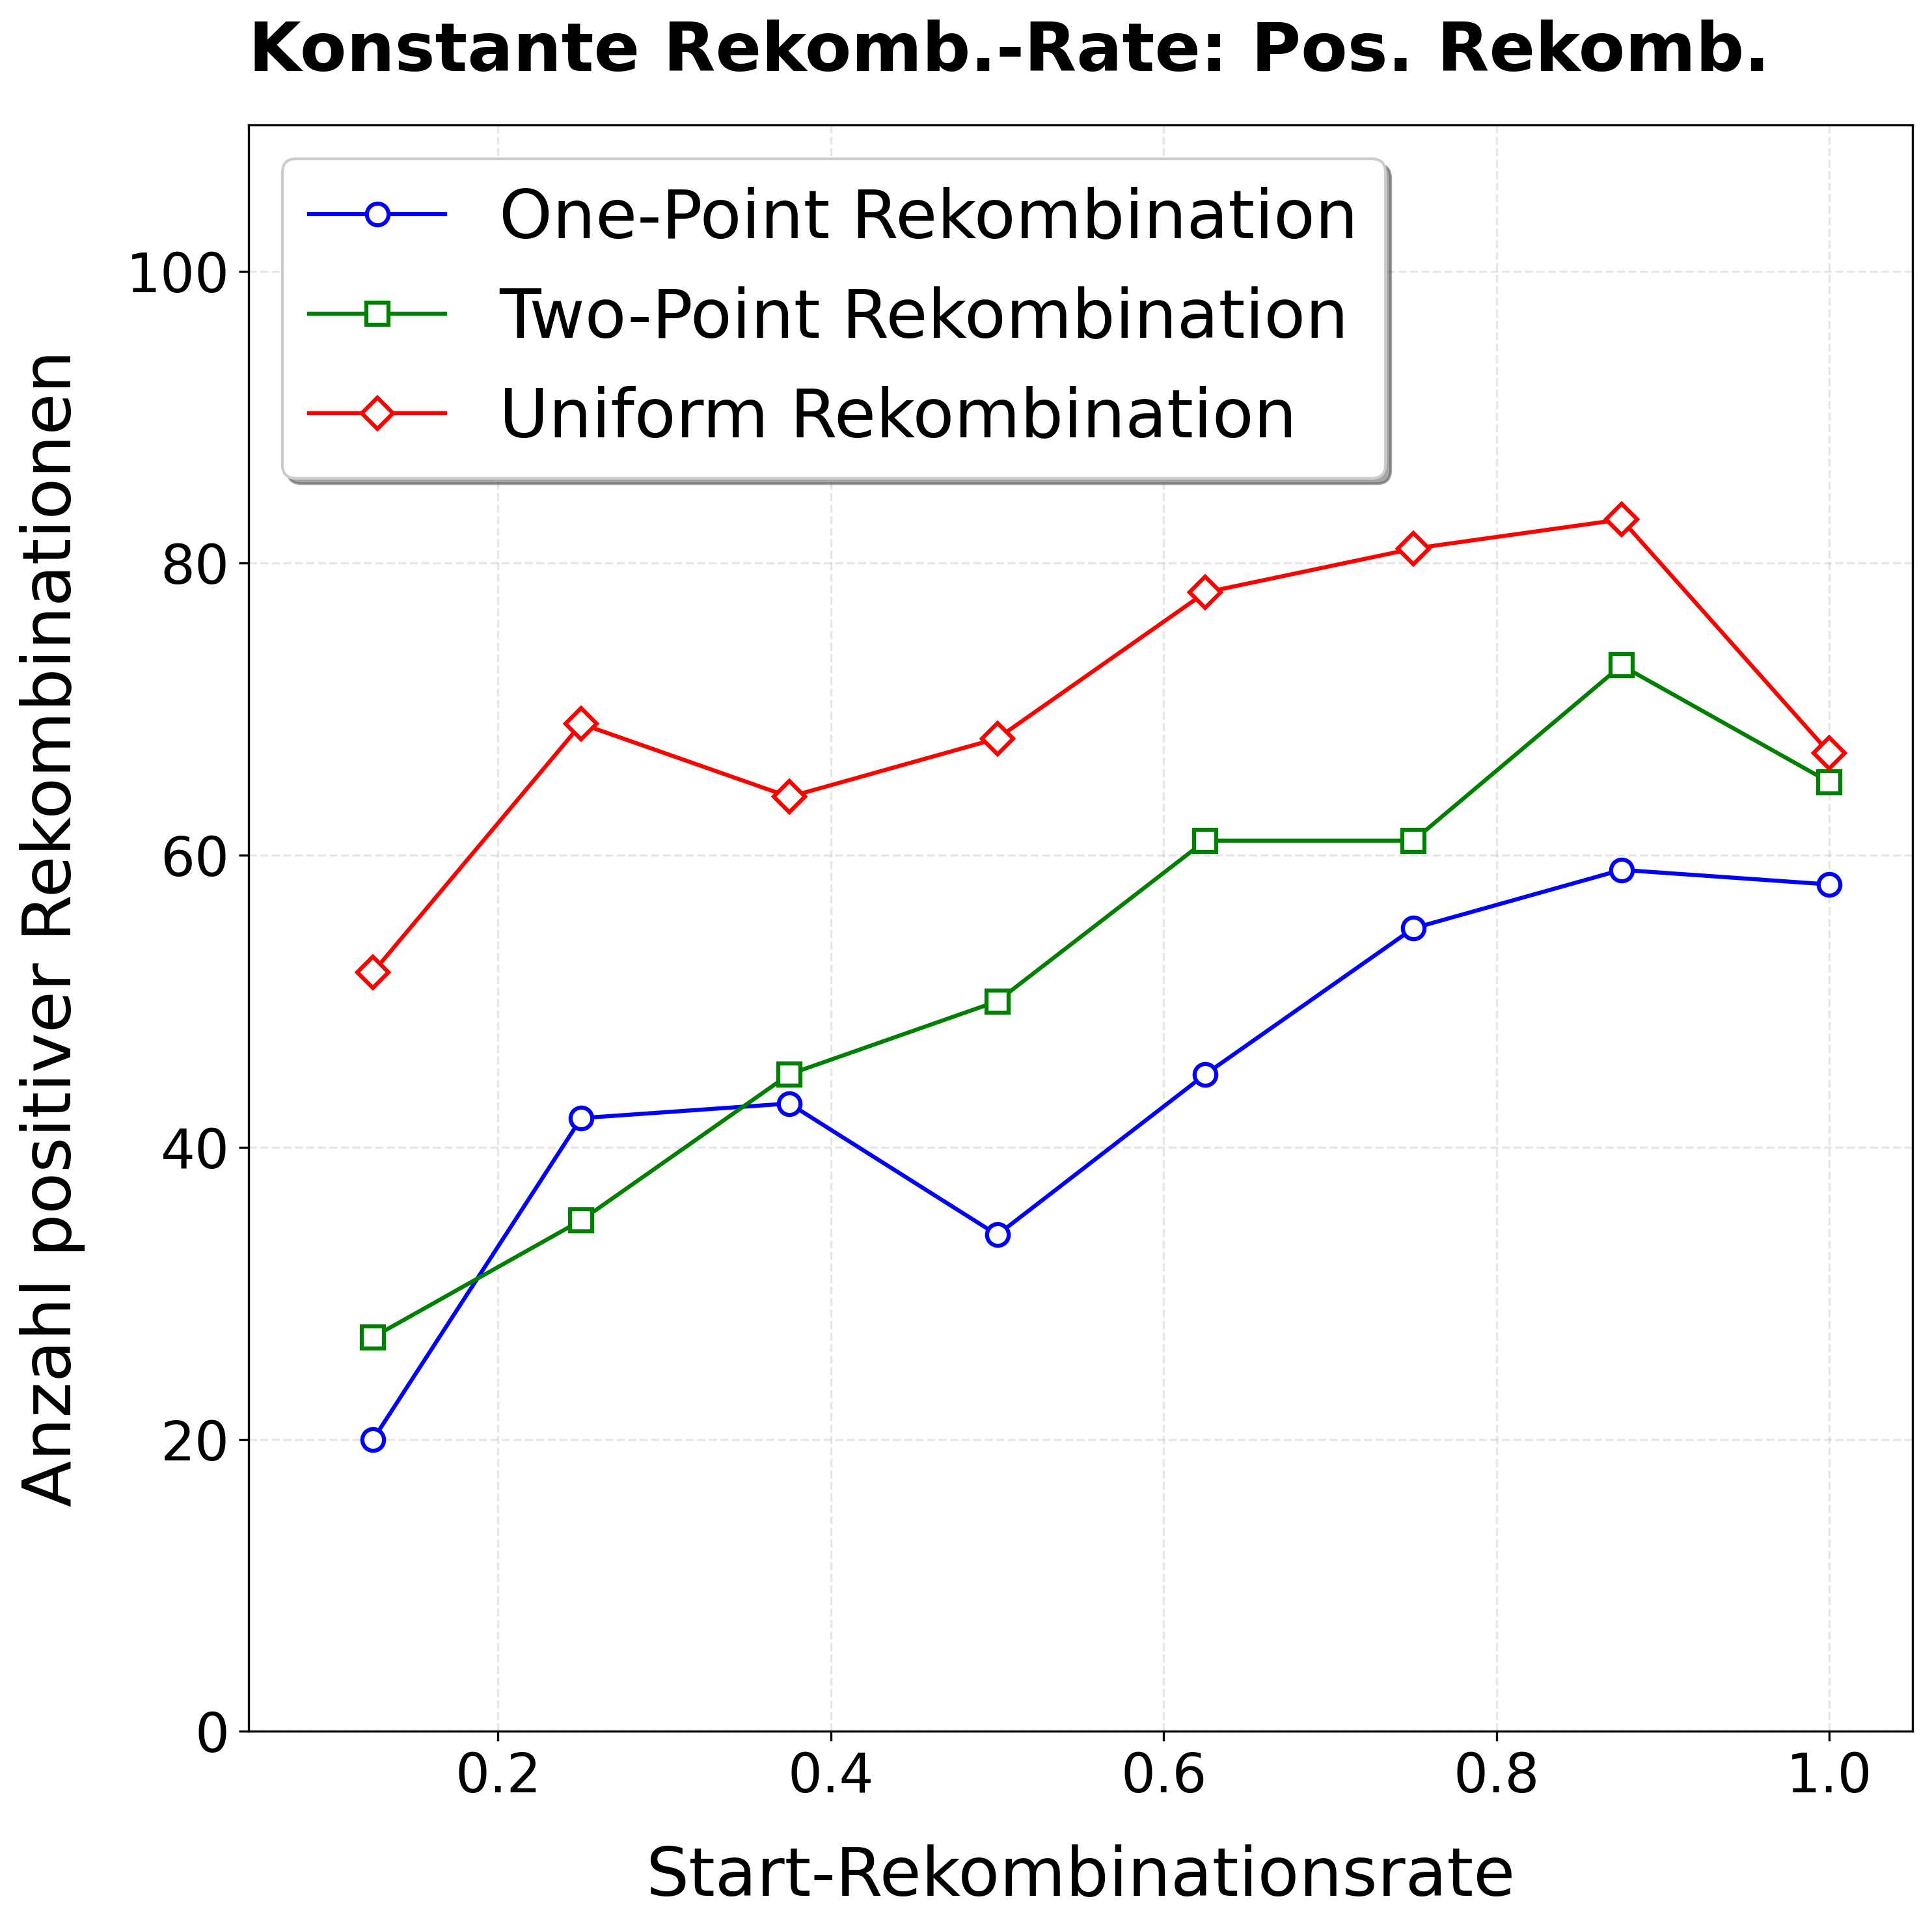
\includegraphics[width=\textwidth]{Bilder/EncodePlotPositiveRekombinationKonstant.png}
		\caption{Konstant}
		\label{fig:encodePosRekombinationKonstant}
	\end{subfigure}%
	\hfill
	\begin{subfigure}[b]{0.32\textwidth}
		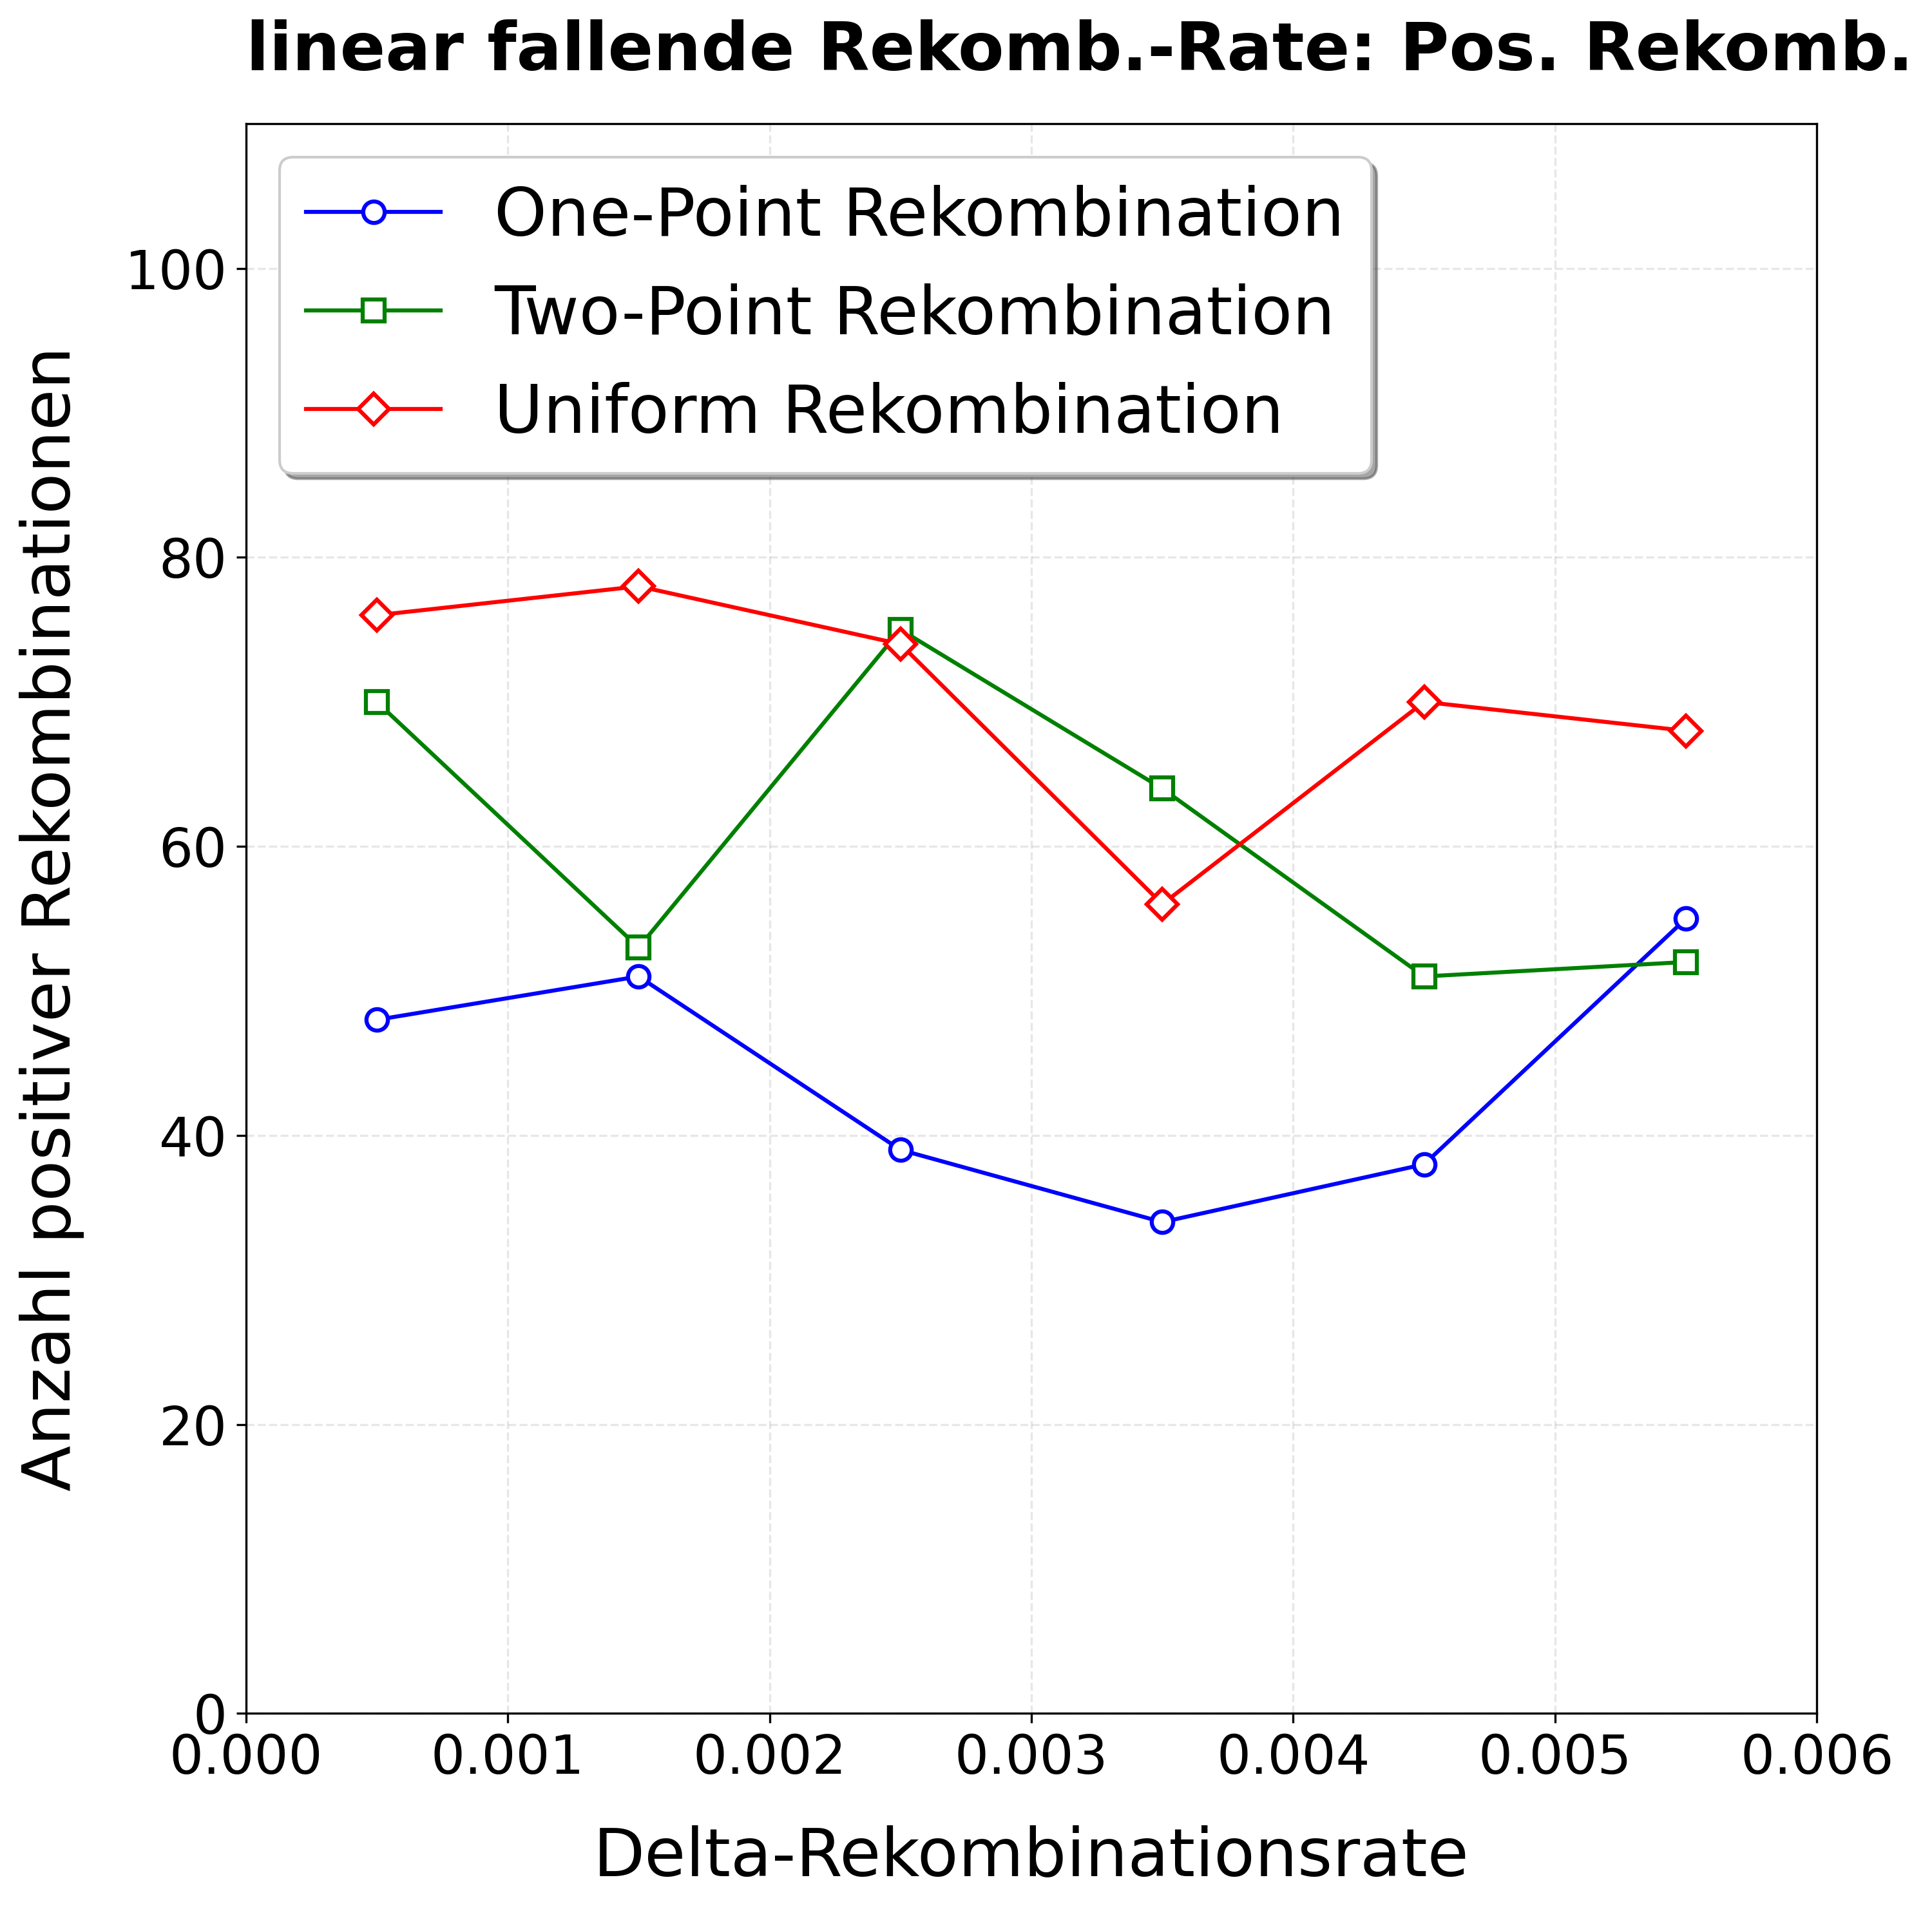
\includegraphics[width=\textwidth]{Bilder/EncodePlotPositiveRekombinationClegg.png}
		\caption{linear fallend}
		\label{fig:encodePosRekombinationClegg}
	\end{subfigure}%
	\hfill
	\begin{subfigure}[b]{0.32\textwidth}
		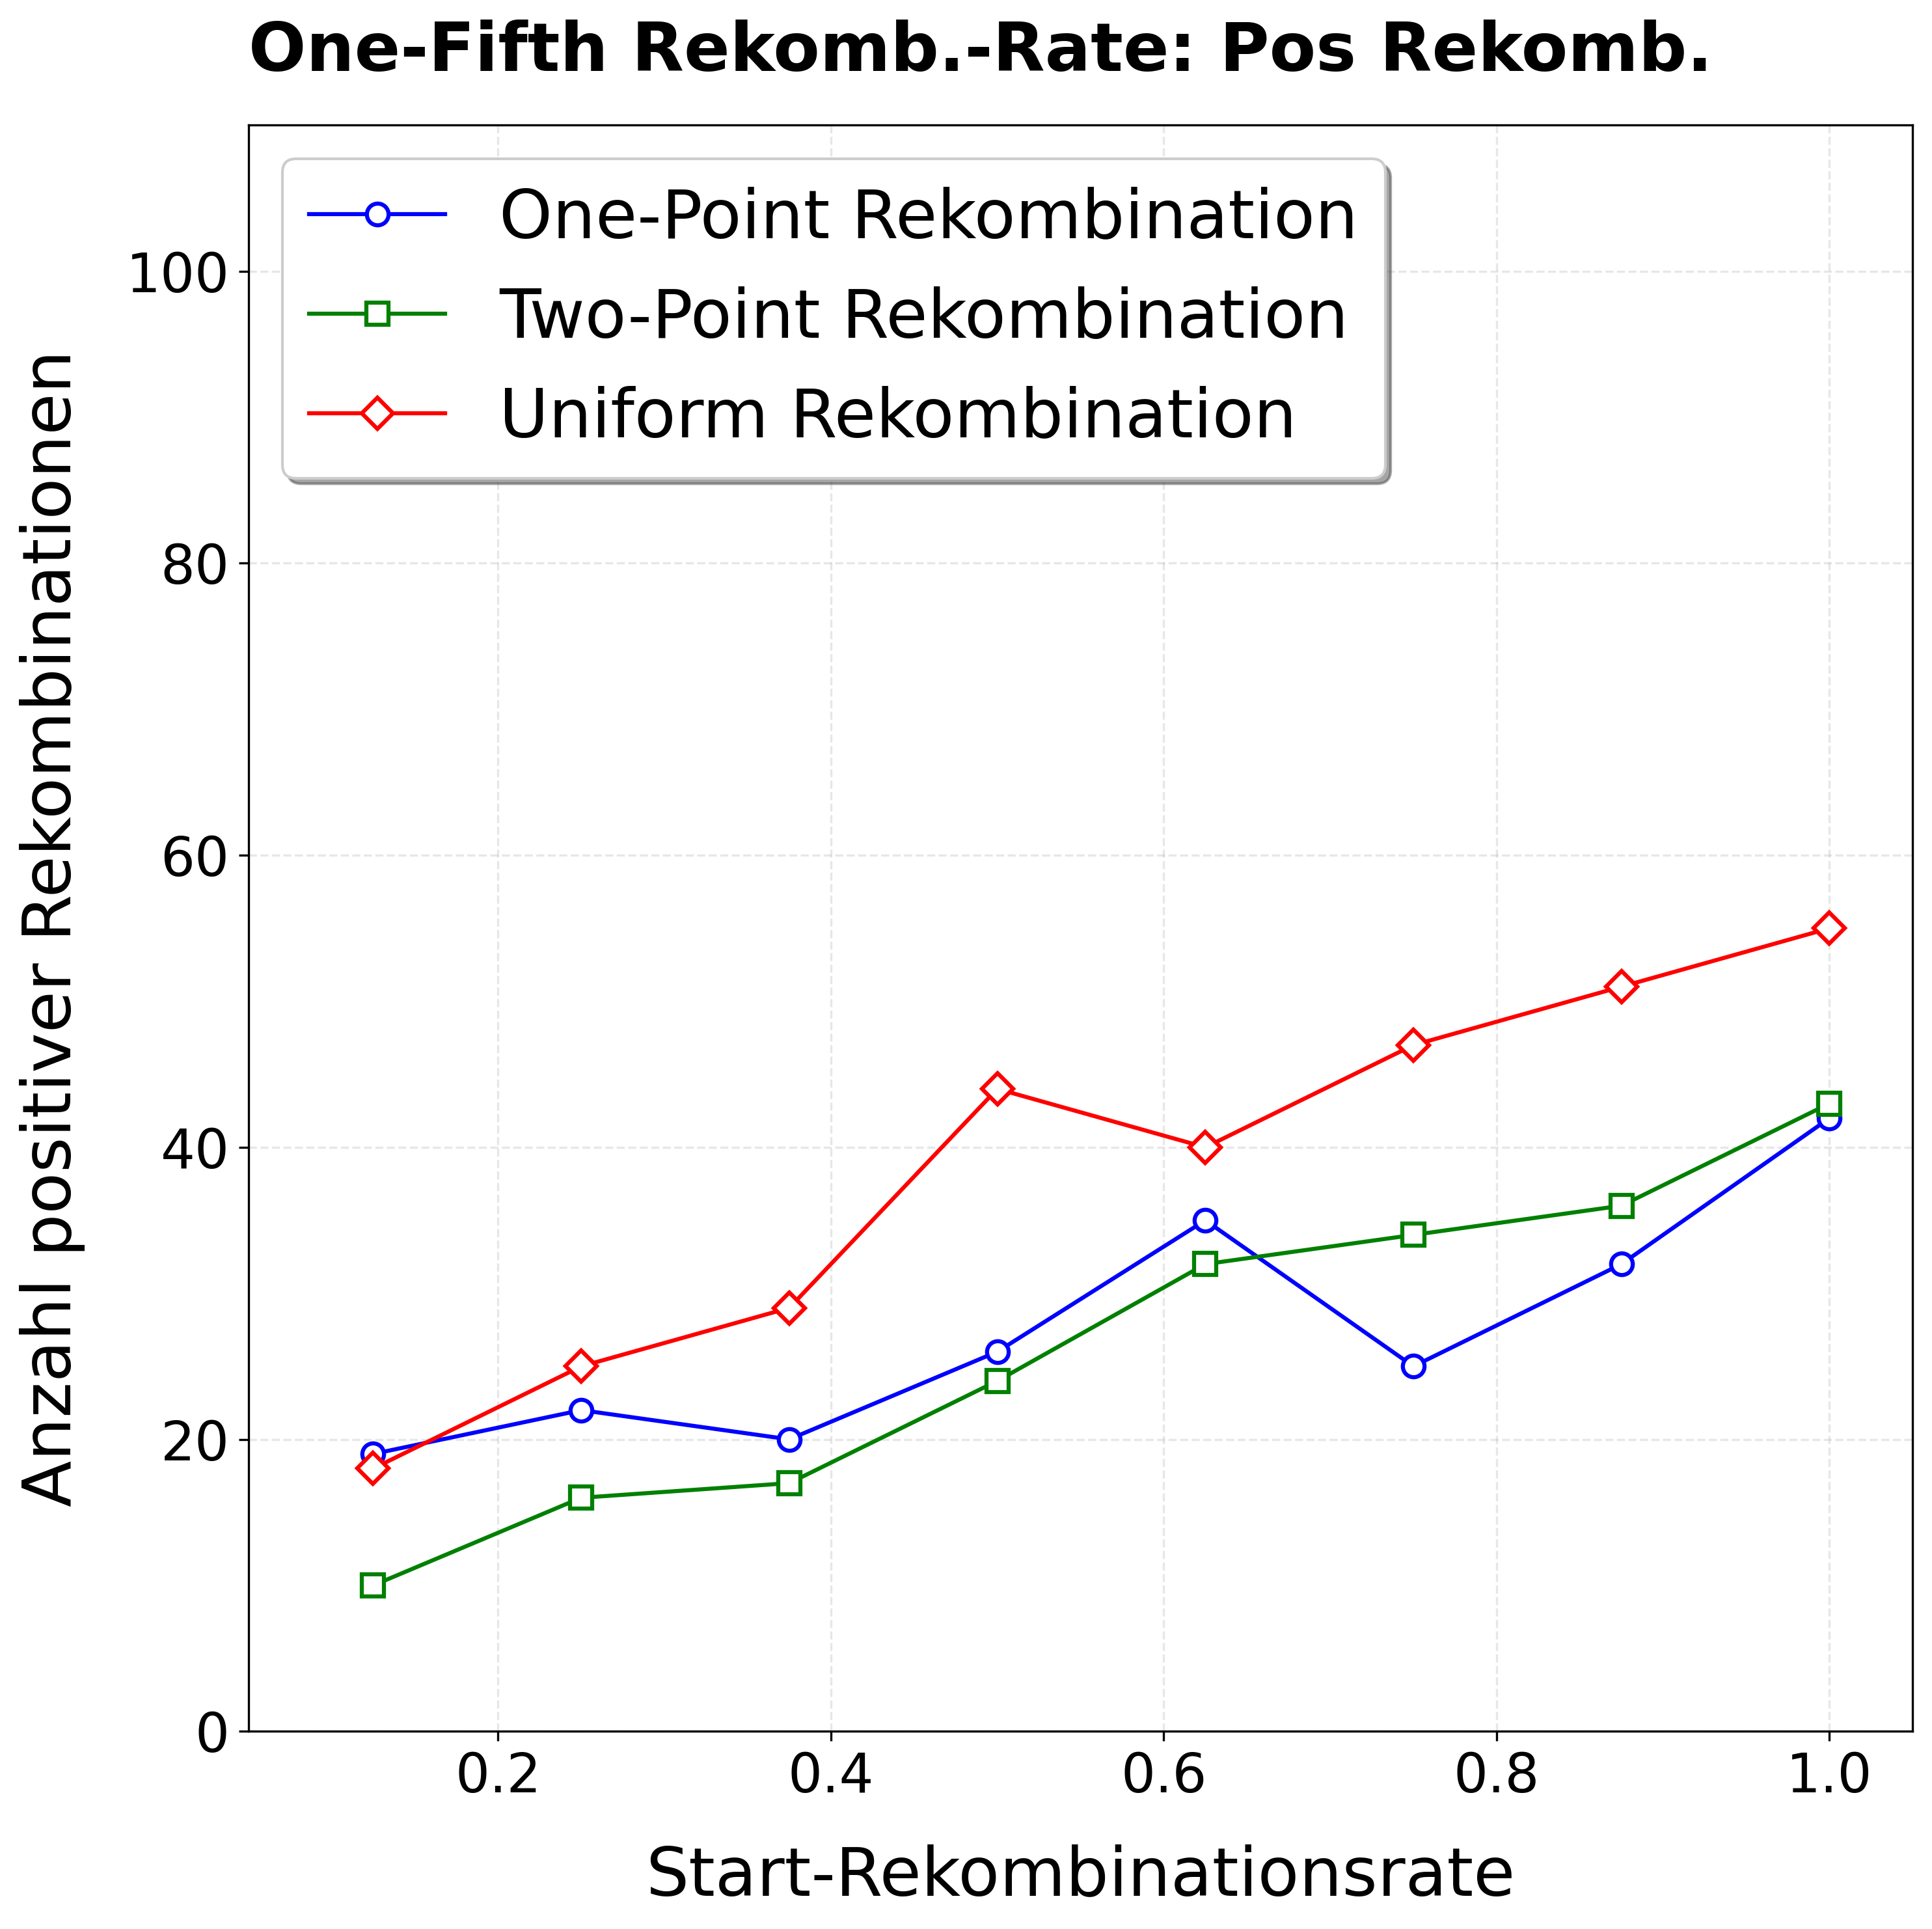
\includegraphics[width=\textwidth]{Bilder/EncodePlotPositiveRekombinationOneFifth.png}
		\caption{One-Fifth Regel}
		\label{fig:encodePosRekombinationOneFifth}
	\end{subfigure}
	\caption{Encode: Raten-Arten und Anzahl positive Rekombinationen}
	\label{fig:encodePosRekombination}
\end{figure}

In Abbildung \ref{fig:encodePosRekombination} kann beobachtet werden, dass für jede Rekombinationsraten-Art die Uniform Rekombination die höchsten Anzahlen an positiver Rekombination produziert.
Für die konstante und linear fallende Rekombinationsrate ist die Two-Point Rekombination in dieser Hinsicht besser als die One-Point Rekombination.
Auch wird ersichtlich, dass die Rekombinationsrate mit der One-Fifth Regel niedrigere Rekombinationserfolge einfährt als die anderen Rekombinationsraten-Arten.\\
Eine höhere Rekombinationsrate bedeutet auch eine höhere Chance, dass die Rekombination ausgeführt wird und somit die Fitness verbessert.
So ist es nicht überraschend, dass die Abbildungen \ref{fig:encodePosRekombinationKonstant} und \ref{fig:encodePosRekombinationOneFifth} insgesamt eine positive Steigung aufzeigen.
Nicht ersichtlich ist allerdings, wieso die konstanten Rekombinationsraten gleich 1,0 weniger gute Ergebnisse liefern als die konstanten Rekombinationsraten gleich 0,875.
Dies gilt für alle Rekombinationsarten mit der konstanten Rekombinationsrate.\\
Ebenfalls überraschend sind die kurzfristigen lokalen Maxima, die die Abbildungen \ref{fig:encodePosRekombinationKonstant} und \ref{fig:encodePosRekombinationOneFifth} bei geringen Rekombinationsraten aufzeigen.
Die hohen Anzahlen an positiven Rekombinationen, obwohl die Rekombination nicht wahrscheinlich ausgeführt wird, könnte darauf hindeuten, dass die ausgeführten Rekombinationsschritte effektiver waren als diejenigen Rekombinationsschritte, die häufiger ausgeführt werden.


\subsection{Rohdatenanalyse: Koza}
\label{subsec:rohdatenKoza}

Die folgenden Tabellen \ref{table:kozaOnePointRohdaten}, \ref{table:kozaTwoPointRohdaten} und \ref{table:kozaUniformRohdaten} zeigen die Rohdaten-Auswertungen des Koza-Testszenarios.
Für jede CGP-Konfiguration wurden 50 Modelle innerhalb von maximal 50000 Iterationen trainiert.
Jede der Tabellen stellt eine Rekombinationsart mit verschiedenen Parametrierungen der Rekombinationsraten dar.
Wie in Abschnitt \ref{subsec:rohdatenEncode} wurde für das Koza-Testszenario der Offset als Parameter ausgestellt.
Dies geht aus den Ergebnissen von Parity und Keijzer hervor, bei denen keine erfolgreichen Rekombinationsschritte ausgeführt wurden, wenn ein Offset aktiv war.
Ziel des Abschnittes ist es die Zusammenhänge zwischen verschiedenen Rekombinationsraten-Arten und dem Erfolg des CGP-Trainings zu finden.
Außerdem soll bestimmt werden, welche Metrik für die Auswertung der bayes'schen Analyse verwendet werden soll.
In diesem Abschnitt werden nur die Ergebnisse von Koza ausgewertet und erlauben noch keine allgemeinen Aussagen.
Diese werden in Abschnitt \ref{subsec:rohdatenZusammenfassung} ausgewertet, indem die Ergebnisse aus allen Testszenarien zusammengetragen und verglichen werden.


\begin{table}[H]
	\centering
	\begin{tabular}{c | c | c | c | c | c | c}
		\begin{turn}{270} \textbf{CGP-Konfigurationen} \end{turn} & \begin{turn}{270} \textbf{Anzahl pos. Mutationen} \end{turn} & \begin{turn}{270} \textbf{Anzahl pos. Rekomb.} \end{turn} & \begin{turn}{270} \textbf{Anzahl neg. Mutationen} \end{turn} & \begin{turn}{270} \textbf{Median Iter. pos. Rekomb.} \end{turn} & \begin{turn}{270} \textbf{Median Iter. bis Konv.} \end{turn} & \begin{turn}{270} \textbf{Stopp-Kriterium erfüllt} \end{turn}\\
		\hline
		keine Rekombination & 1157 & - & - & - & 208 & 48\\
		\hline
		One-Point Konstant: 0,125 & 1338 & 9 & 8 & 42 & 616 & 41\\
		\hline
		One-Point Konstant: 0,25 & 1180 & 23 & 16 & 7 & 611 & 45\\
		\hline
		One-Point Konstant: 0,375 & 1493 & 42 & 25 & 43 & 2012 & 47\\
		\hline
		One-Point Konstant: 0,5 & 1477 & 57 & 40 & 18 & 602,5 & 36\\
		\hline
		One-Point Konstant: 0,625 & 1287 & 48 & 23 & 82,5 & 2302 & 45\\
		\hline
		One-Point Konstant: 0,75 & 1423 & 65 & 43 & 29 & 989 & 47\\
		\hline
		One-Point Konstant: 0,875 & 1593 & 85 & 48 & 18 & 848 & 34\\
		\hline
		One-Point Konstant: 1,0 & 1548 & 136 & 83 & 73,5 & 667 & 41\\
		\hline
		One-Point Clegg: 0,0005 & 1460 & 98 & 56 & 45,5 & 603 & 43\\
		\hline
		One-Point Clegg: 0,0015 & 1525 & 78 & 43 & 12 & 659 & 40\\
		\hline
		One-Point Clegg: 0,0025 & 1303 & 52 & 31 & 7 & 583 & 41\\
		\hline
		One-Point Clegg: 0,0035 & 1233 & 61 & 35 & 6 & 529 & 42\\
		\hline
		One-Point Clegg: 0,0045 & 1187 & 62 & 36 & 10 & 511 & 44\\
		\hline
		One-Point Clegg: 0,0055 & 1622 & 50 & 28 & 9,5 & 1320 & 42\\
		\hline
		One-Point One-Fifth: 0,125 & 1434 & 2 & 1 & 1,5 & 462 & 44\\
		\hline
		One-Point One-Fifth: 0,25 & 1544 & 7 & 6 & 1 & 1400 & 44\\
		\hline
		One-Point One-Fifth: 0,375 & 1005 & 13 & 8 & 2 & 838,5 & 46\\
		\hline
		One-Point One-Fifth: 0,5 & 1137 & 14 & 10 & 2 & 360,5 & 41\\
		\hline
		One-Point One-Fifth: 0,625 & 1207 & 18 & 12 & 2 & 947 & 44\\
		\hline
		One-Point One-Fifth: 0,75 & 1387 & 17 & 11 & 3 & 910 & 43\\
		\hline
		One-Point One-Fifth: 0,875 & 1160 & 29 & 14 & 4 & 301 & 43\\
		\hline
		One-Point One-Fifth: 1,0 & 1393 & 38 & 25 & 4 & 568 & 43\\
	\end{tabular}
	\caption{Koza One-Point Rekombination: Auswertung der Rohdaten}
	\label{table:kozaOnePointRohdaten}
\end{table}



\begin{table}[H]
	\centering
	\begin{tabular}{c | c | c | c | c | c | c}
		\begin{turn}{270} \textbf{CGP-Konfigurationen} \end{turn} & \begin{turn}{270} \textbf{Anzahl pos. Mutationen} \end{turn} & \begin{turn}{270} \textbf{Anzahl pos. Rekomb.} \end{turn} & \begin{turn}{270} \textbf{Anzahl neg. Mutationen} \end{turn} & \begin{turn}{270} \textbf{Median Iter. pos. Rekomb.} \end{turn} & \begin{turn}{270} \textbf{Median Iter. bis Konv.} \end{turn} & \begin{turn}{270} \textbf{Stopp-Kriterium erfüllt} \end{turn}\\
		\hline
		keine Rekombination & 1157 & - & - & - & 208 & 48\\
		\hline
		Two-Point Konstant: 0,125 & 1383 & 41 & 24 & 106 & 106 & 45\\
		\hline
		Two-Point Konstant: 0,25 & 1475 & 82 & 55 & 47,5 & 613 & 48\\
		\hline
		Two-Point Konstant: 0,375 & 1207 & 91 & 58 & 75 & 153 & 43\\
		\hline
		Two-Point Konstant: 0,5 & 1120 & 85 & 49 & 29 & 194 & 46\\
		\hline
		Two-Point Konstant: 0,625 & 1013 & 93 & 38 & 16 & 124 & 49\\
		\hline
		Two-Point Konstant: 0,75 & 1373 & 145 & 65 & 21 & 190 & 43\\
		\hline
		Two-Point Konstant: 0,875 & 1400 & 140 & 76 & 26 & 731 & 46\\
		\hline
		Two-Point Konstant: 1,0 & 1176 & 220 & 140 & 50,5 & 207 & 48\\
		\hline
		Two-Point Clegg: 0,0005 & 1446 & 193 & 99 & 30 & 205 & 47\\
		\hline
		Two-Point Clegg: 0,0015 & 1167 & 105 & 59 & 14 & 154 & 45\\
		\hline
		Two-Point Clegg: 0,0025 & 1396 & 106 & 53 & 18 & 504,5 & 44\\
		\hline
		Two-Point Clegg: 0,0035 & 1043 & 95 & 45 & 13 & 142 & 46\\
		\hline
		Two-Point Clegg: 0,0045 & 1023 & 100 & 50 & 14,5 & 96 & 46\\
		\hline
		Two-Point Clegg: 0,0055 & 1160 & 94 & 43 & 11,5 & 223,5 & 49\\
		\hline
		Two-Point One-Fifth: 0,125 & 1422 & 5 & 4 & 2 & 226 & 45\\
		\hline
		Two-Point One-Fifth: 0,25 & 1348 & 10 & 5 & 4 & 404,5 & 44\\
		\hline
		Two-Point One-Fifth: 0,375 & 1365 & 15 & 4 & 3 & 460 & 46\\
		\hline
		Two-Point One-Fifth: 0,5 & 1761 & 15 & 4 & 5 & 584 & 47\\
		\hline
		Two-Point One-Fifth: 0,625 & 1165 & 22 & 13 & 6 & 165 & 48\\
		\hline
		Two-Point One-Fifth: 0,75 & 1041 & 26 & 13 & 4 & 213,5 & 46\\
		\hline
		Two-Point One-Fifth: 0,875 & 1050 & 42 & 19 & 7 & 185 & 48\\
		\hline
		Two-Point One-Fifth: 1,0 & 1142 & 35 & 20 & 5 & 348 & 49\\
	\end{tabular}
	\caption{Koza Two-Point Rekombination: Auswertung der Rohdaten}
	\label{table:kozaTwoPointRohdaten}
\end{table}




\begin{table}[H]
	\centering
	\begin{tabular}{c | c | c | c | c | c | c}
		\begin{turn}{270} \textbf{CGP-Konfigurationen} \end{turn} & \begin{turn}{270} \textbf{Anzahl pos. Mutationen} \end{turn} & \begin{turn}{270} \textbf{Anzahl pos. Rekomb.} \end{turn} & \begin{turn}{270} \textbf{Anzahl neg. Mutationen} \end{turn} & \begin{turn}{270} \textbf{Median Iter. pos. Rekomb.} \end{turn} & \begin{turn}{270} \textbf{Median Iter. bis Konv.} \end{turn} & \begin{turn}{270} \textbf{Stopp-Kriterium erfüllt} \end{turn}\\
		\hline
		keine Rekombination & 1157 & - & - & - & 208 & 48\\
		\hline
		Uniform Konstant: 0,125 & 1178 & 124 & 75 & 31,5 & 316 & 44\\
		\hline
		Uniform Konstant: 0,25 & 1233 & 157 & 90 & 44 & 479 & 43\\
		\hline
		Uniform Konstant: 0,375 & 1166 & 251 & 132 & 35 & 257,5 & 47\\
		\hline
		Uniform Konstant: 0,5 & 1084 & 184 & 92 & 27,5 & 113 & 45\\
		\hline
		Uniform Konstant: 0,625 & 1277 & 295 & 152 & 31 & 430 & 47\\
		\hline
		Uniform Konstant: 0,75 & 1301 & 276 & 141 & 31 & 382 & 43\\
		\hline
		Uniform Konstant: 0,875 & 1102 & 332 & 181 & 31 & 467 & 44\\
		\hline
		Uniform Konstant: 1,0 & 1080 & 328 & 199 & 21 & 176 & 43\\
		\hline
		Uniform Clegg: 0,0005 & 1155 & 373 & 197 & 40 & 709 & 46\\
		\hline
		Uniform Clegg: 0,0015 & 793 & 259 & 147 & 17 & 81 & 48\\
		\hline
		Uniform Clegg: 0,0025 & 887 & 319 & 181 & 25 & 140 & 48\\
		\hline
		Uniform Clegg: 0,0035 & 1415 & 318 & 162 & 18 & 162 & 46\\
		\hline
		Uniform Clegg: 0,0045 & 1404 & 304 & 153 & 18 & 637 & 48\\
		\hline
		Uniform Clegg: 0,0055 & 1364 & 300 & 141 & 19 & 143 & 46\\
		\hline
		Uniform One-Fifth: 0,125 & 1545 & 12 & 6 & 5 & 147 & 41\\
		\hline
		Uniform One-Fifth: 0,25 & 1314 & 24 & 8 & 6 & 153 & 44\\
		\hline
		Uniform One-Fifth: 0,375 & 1384 & 36 & 14 & 8,5 & 273 & 47\\
		\hline
		Uniform One-Fifth: 0,5 & 1718 & 61 & 28 & 6 & 848 & 46\\
		\hline
		Uniform One-Fifth: 0,625 & 1244 & 72 & 35 & 6 & 363 & 47\\
		\hline
		Uniform One-Fifth: 0,75 & 1320 & 90 & 49 & 5 & 207 & 44\\
		\hline
		Uniform One-Fifth: 0,875 & 1406 & 92 & 49 & 9 & 470 & 46\\
		\hline
		Uniform One-Fifth: 1,0 & 1444 & 83 & 40 & 6 & 794,5 & 47\\
	\end{tabular}
	\caption{Koza Uniform Rekombination: Auswertung der Rohdaten}
	\label{table:kozaUniformRohdaten}
\end{table}

Aus den Spalten \glqq Stopp-Kriterium erfüllt\grqq\space der drei Tabellen \ref{table:kozaOnePointRohdaten}, \ref{table:kozaTwoPointRohdaten} und \ref{table:kozaUniformRohdaten} geht hervor, dass relativ viele Durchgänge des CGP-Trainings konvergiert sind.
Deswegen wird für die bayes'sche Analyse in Abschnitt \ref{subsec:bayesKoza} die Anzahl an Iterationen bis zur Konvergenz als Metrik verwendet.
Außerdem lässt sich erkennen, dass mehr Mutationen zu einer Verbesserung der Fitness geführt haben als es die Rekombinationsschritte getan haben.
Gleichzeitig werden einige Erfolge der Rekombinationsschritte verloren, indem anschließend noch eine Mutation ausgeführt wurde, wie in den Spalten \glqq Anzahl negative Mutationen\grqq\space zu sehen ist.
Dies kann dadurch passieren, dass die Auswahl der Elitisten erst nach der Mutation getroffen wird und so keine Evaluation der Fitness zwischen Rekombination und Mutation stattfindet.
Eine Möglichkeit dies zu beheben wäre es, die Elitisten nach der Rekombination mit den Elitisten nach der Mutation abzugleichen und so die besten Chromosomen zu verwenden, die aus beiden genetischen Operationen resultieren.\\
Die Rekombination ist dabei vor allem in den frühen Iterationen erfolgreich.
Dabei unterscheiden sich die unterschiedlichen Rekombinationsraten-Arten.
Die Rekombination mit der One-Fifth Regel weist vor allem in den ersten Iterationen Erfolge auf, mit der linear fallenden Rekombinationsrate ist der Median etwas höher und mit der konstanten Rekombinationsrate sind teilweise relativ hohe Iterationen noch erfolgreich.
Für die konstante Rekombinationsrate werden diese hohen Iterationsmediane allerdings nur für die One-Point und Two-Point Rekombination gesichtet.
Dabei fällt auf, dass diese späten Rekombinationserfolge im Training nicht im Zusammenhang mit der Höhe der Rekombinationsrate stehen, da einige erhöhte Werte in den Spalten \glqq Median Iterationen positive Rekombination\grqq\space auch für kleinere Rekombinationsraten auftauchen.
Außerdem kann kein Zusammenhang zwischen den Spalten \glqq Median Iterationen positive Rekombination\grqq\space und \glqq Median Iterationen bis Konvergenz\grqq\space gefunden werden.
Das bedeutet, dass die Rekombinationserfolge nicht durch längeres Training automatisch auch zu späteren Iterationen stattfinden, sondern dass dieses Verhalten unabhängig von der Trainingsdauer auftritt.
Dieses Wissen könnte genutzt werden, um so Rekombination gezielter einzusetzen.
Beispielsweise könnte man die frühen Rekombinationserfolge der linear fallenden Rekombinationsrate nutzen, wobei diese ähnlich viele positive Rekombinationen aufweist wie die konstante Rekombinationsrate.
So könnte man in den ersten Iterationen die Erfolge der Rekombination nutzen und anschließend die Rekombinationsrate schneller reduzieren.\\
Werden die Iterationen betrachtet, die die Modelle bis zur Konvergenz gebraucht haben, lässt sich feststellen, dass die CGP-Modelle mit Two-Point Rekombination durchschnittlich weniger Iterationen (278) gebraucht hat als die anderen.
Darauf folgt die Uniform Rekombination (349 Iterationen) und anschließend die One-Point Rekombination (835 Iterationen).
Demnach sind alle Mittelwerte der Iterationsmediane bis zur Konvergenz größer als der Median der Anzahl an Iterationen, die das CGP-Modell ohne Rekombination gebraucht hat (208).
Dabei muss allerdings beachtet werden, dass bei der CGP-Konfiguration ohne Rekombination alle Hyperparameter optimiert wurden.
Demnach liefern die CGP-Modelle ohne Rekombination optimierte Ergebnisse während alle anderen CGP-Konfigurationen dieses Potential noch ausschöpfen können.
Trotzdem können für einige vereinzelte CGP-Konfigurationen bereits frühere Konvergenzen bei gleicher Anzahl an erfüllten Stopp-Kriterien beobachtet werden.
Ein Beispiel bietet die Konfiguration \glqq Uniform Clegg: 0,0015\grqq\space aus Tabelle \ref{table:kozaUniformRohdaten}.
Dies ist ein Anzeichen dafür, dass CGP-Modelle durch Rekombination effizienter werden können, wenn die Rekombination sinnvoll eingesetzt wird.\\
Des weiteren wurde beim Vergleich der Spalten \glqq Anzahl positive Rekombinationen\grqq, \glqq Anzahl negative Mutationen\grqq\space und \glqq Median Iterationen positive Rekombinationen\grqq mit den Spalten \glqq Median Iterationen bis Konvergenz\grqq\space und \glqq Stopp-Kriterium erfüllt\grqq\space keine zusammenhängenden Muster erkannt.
Eine Möglichkeit dafür, dass die Anzahl der positiven Rekombinationen keine deutliche Veränderungen in der Effizienz des CGPs hervorruft, könnten die negativen Mutationen sein.
In weiteren Tests könnte dieser Zusammenhang untersucht werden, indem keine Mutation ausgeführt wird, wenn bereits eine Rekombination die Fitness des Modells verbessert hat.
So könnte überprüft werden, ob die CGP-Modelle mit mehr Rekombinationserfolgen auch bessere Ergebnisse liefern oder ob Mutationserfolge relevanter für ein erfolgreiches CGP-Training sind.\\
Ein weiterer Punkt der auffällt sind die relativ hohen Zahlen der negativen Mutationen im Koza-Testszenario.
Dies könnte daran liegen, dass die Fitness-Werte in SR Benchmarks kontinuierlich sind, während sie in booleschen Problemen durch diskrete Werte abgebildet werden.
Dadurch können auch kleinere Trainingserfolge durch Rekombination in den Tabellen abgebildet werden.
Dies könnte bedeuten, dass vor allen bei SR die Evaluierung nach der Rekombination als Zwischenschritt sinnvoll sein könnte.\\
Um die positiven Rekombinationen zu bewerten wird folgende Abbildung \ref{fig:kozaPosRekombination} eingeführt:

\begin{figure}[H]
	\centering
	\begin{subfigure}[b]{0.32\textwidth}
		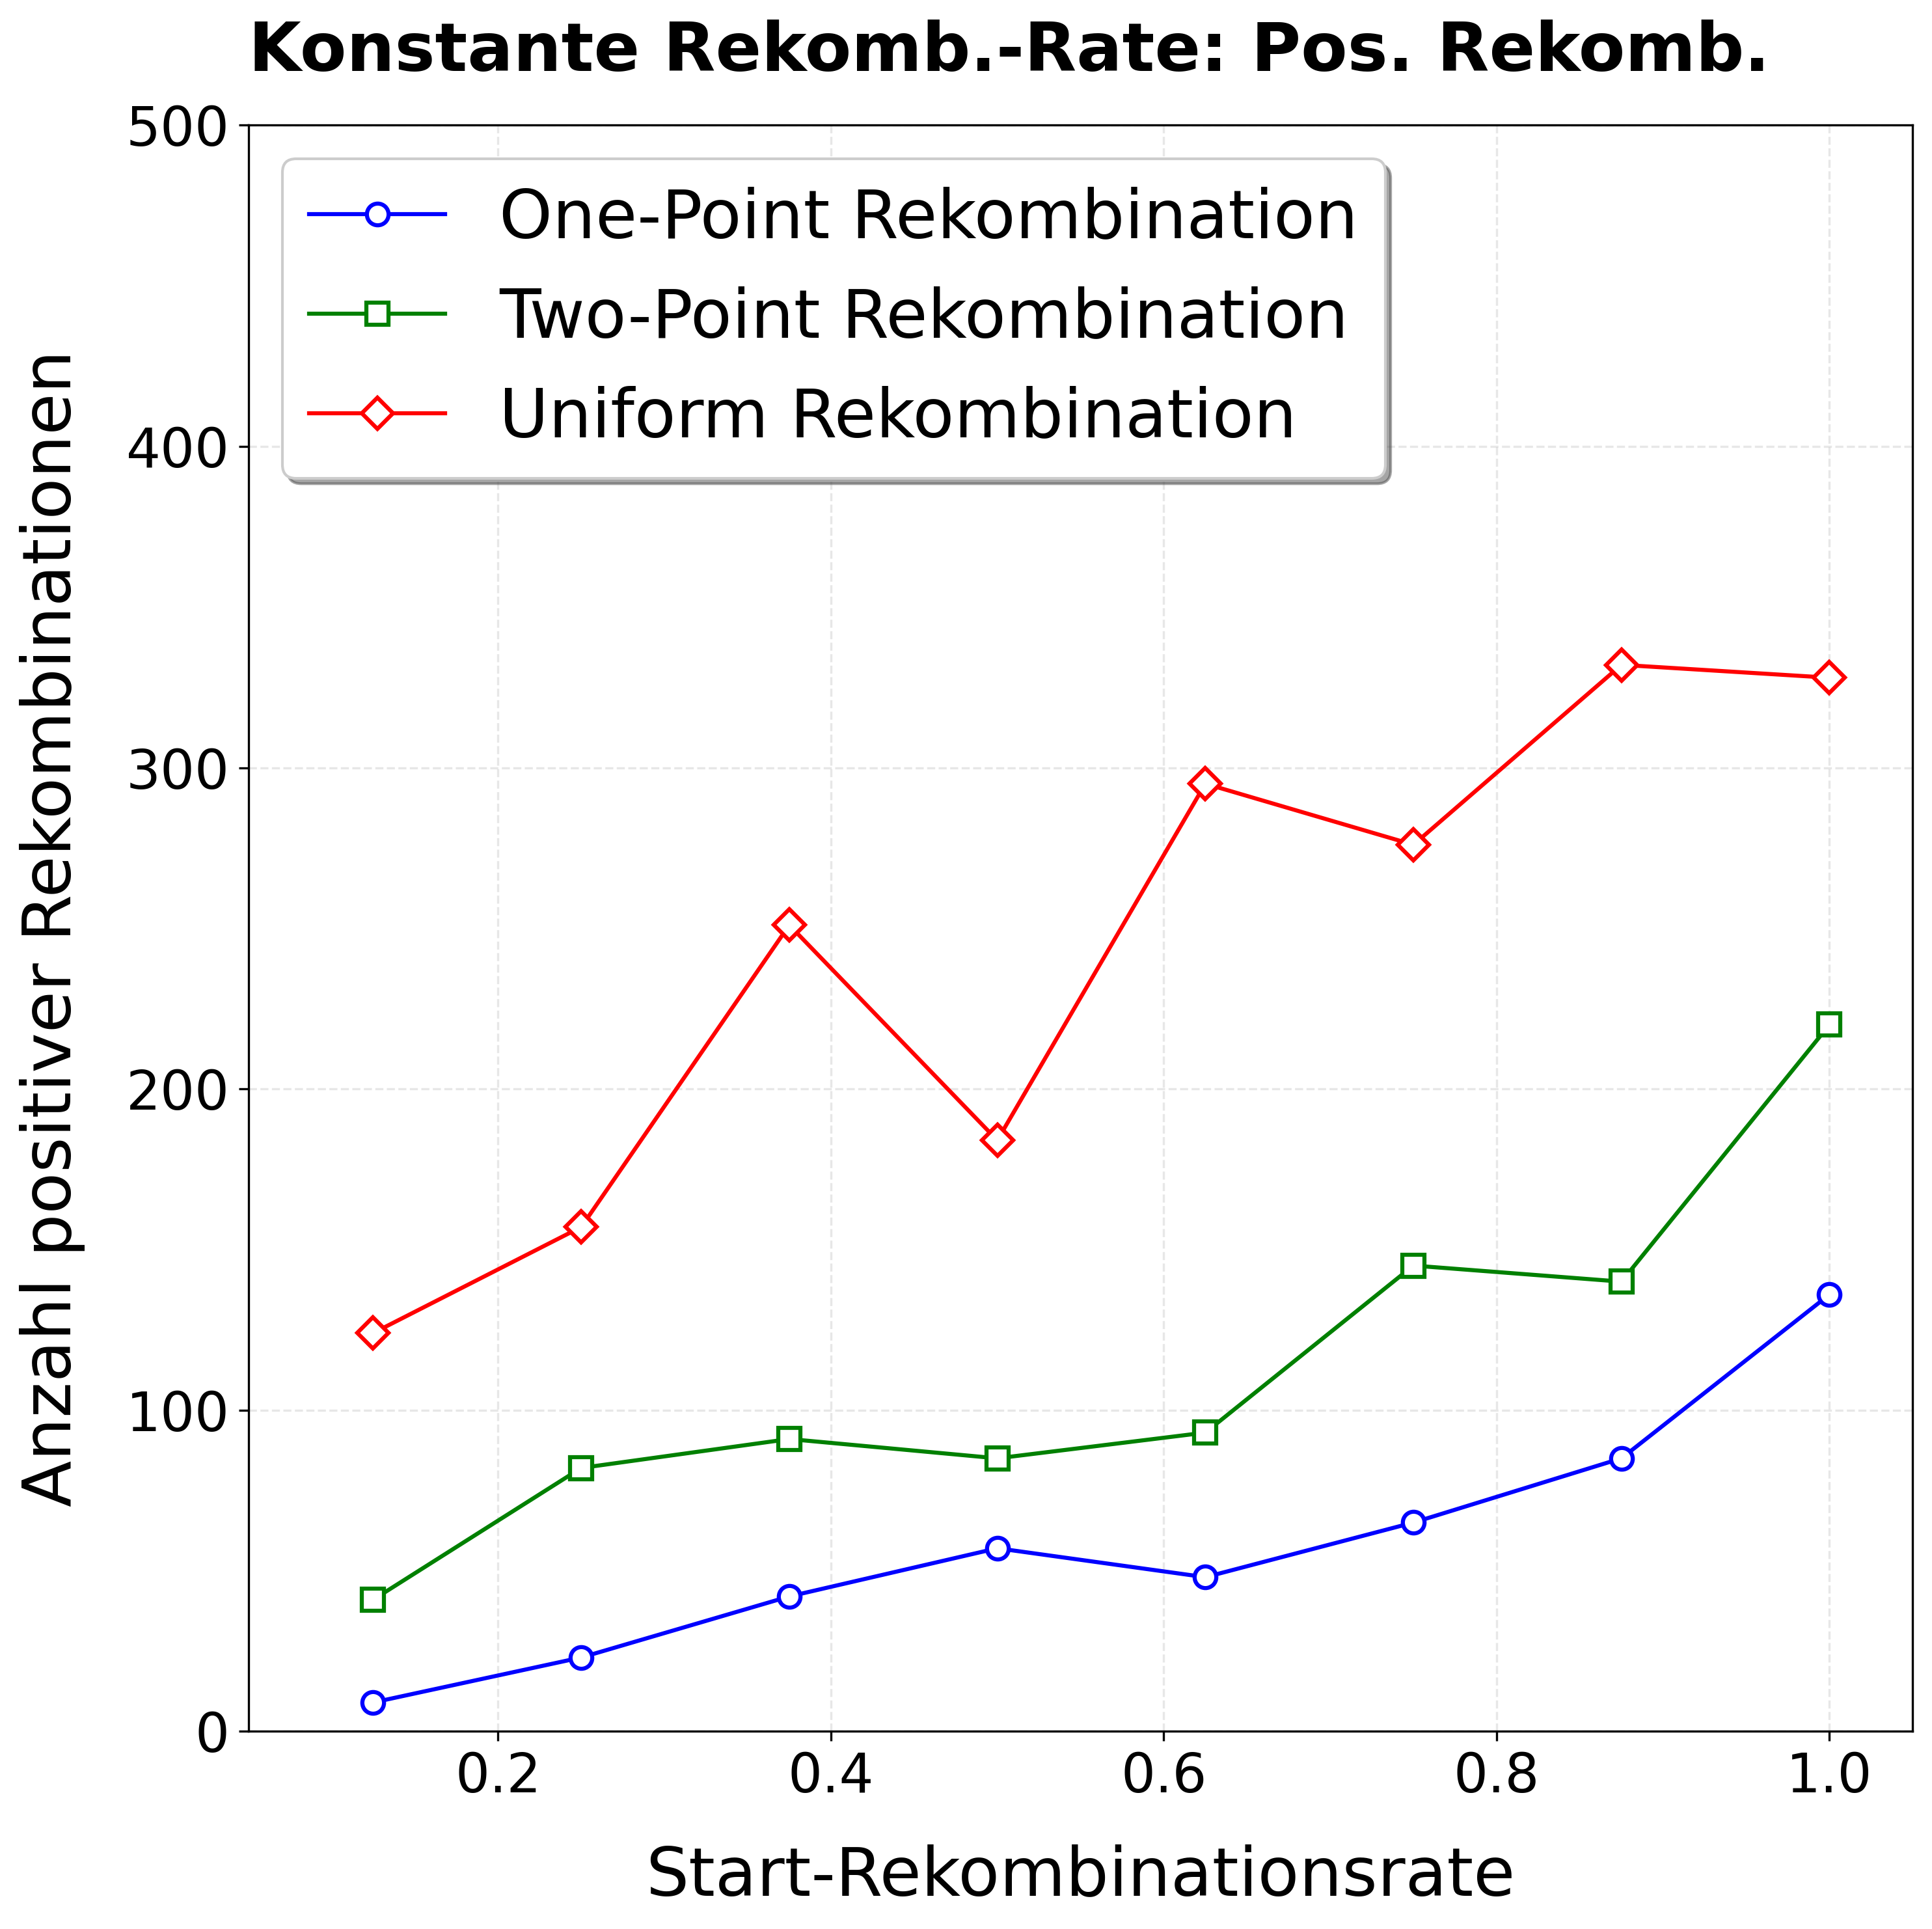
\includegraphics[width=\textwidth]{Bilder/KozaPlotPositiveRekombinationKonstant.png}
		\caption{Konstant}
		\label{fig:kozaPosRekombinationKonstant}
	\end{subfigure}%
	\hfill
	\begin{subfigure}[b]{0.32\textwidth}
		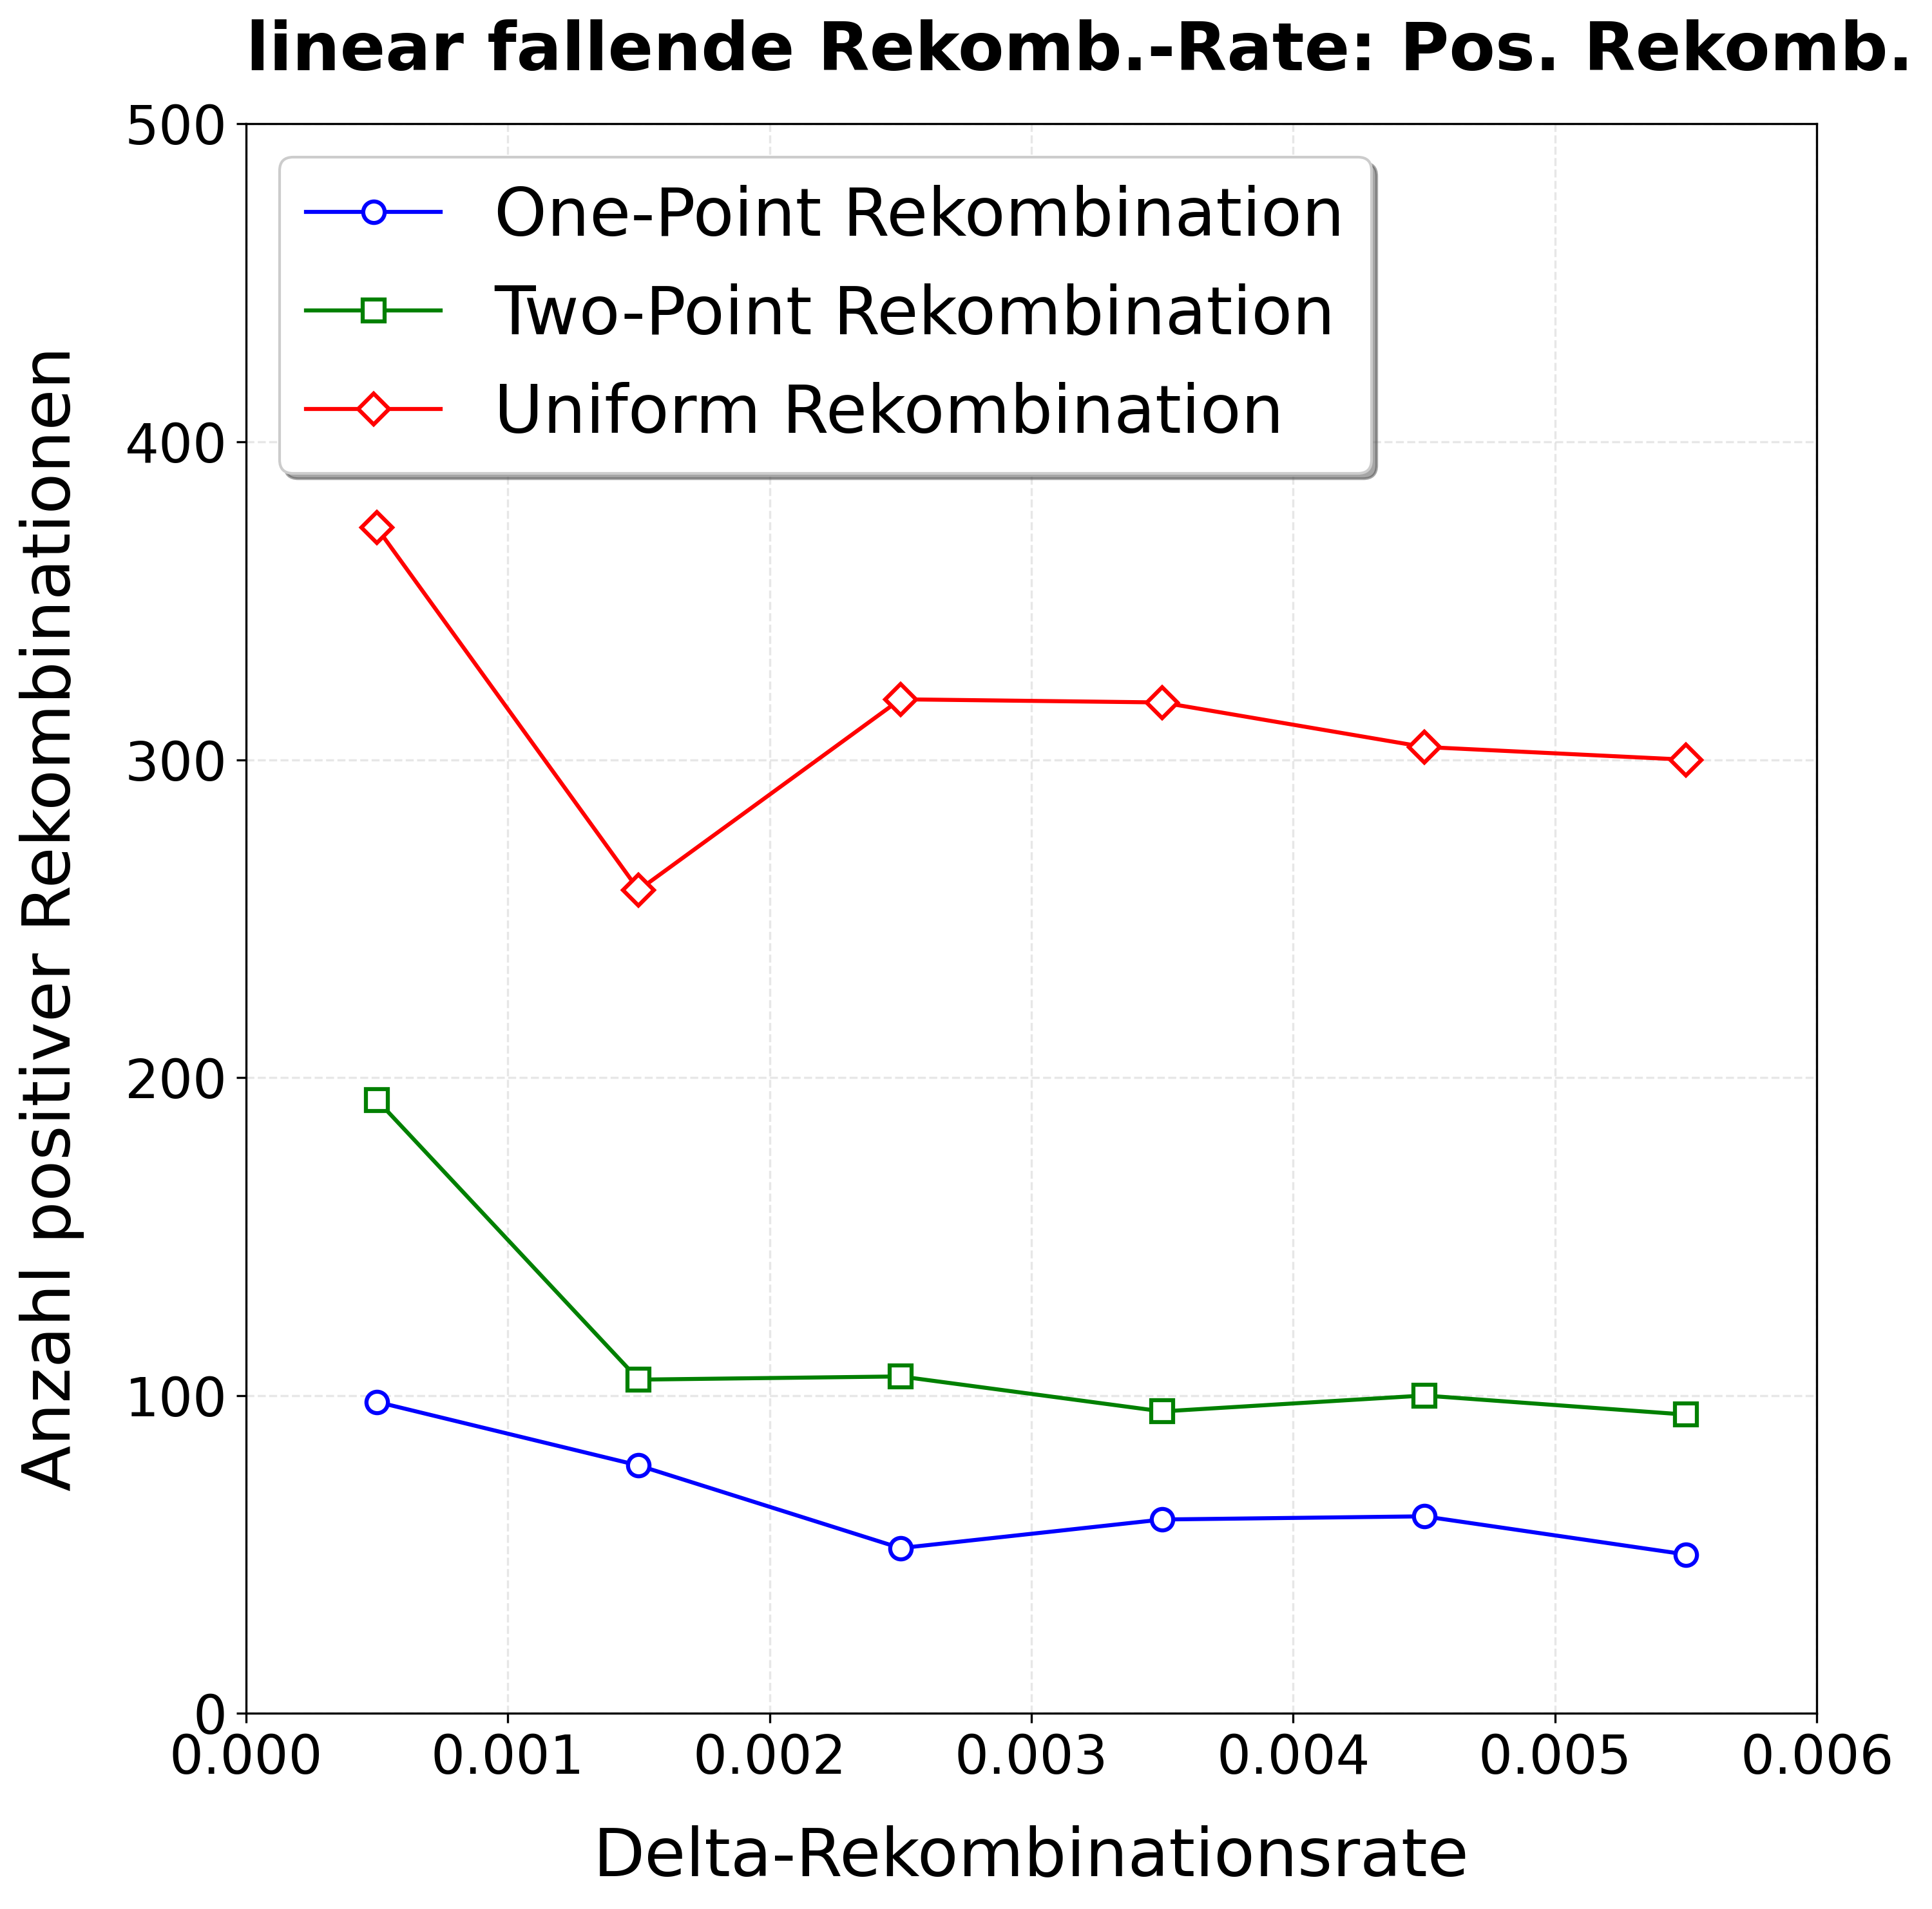
\includegraphics[width=\textwidth]{Bilder/KozaPlotPositiveRekombinationClegg.png}
		\caption{linear fallend}
		\label{fig:kozaPosRekombinationClegg}
	\end{subfigure}%
	\hfill
	\begin{subfigure}[b]{0.32\textwidth}
		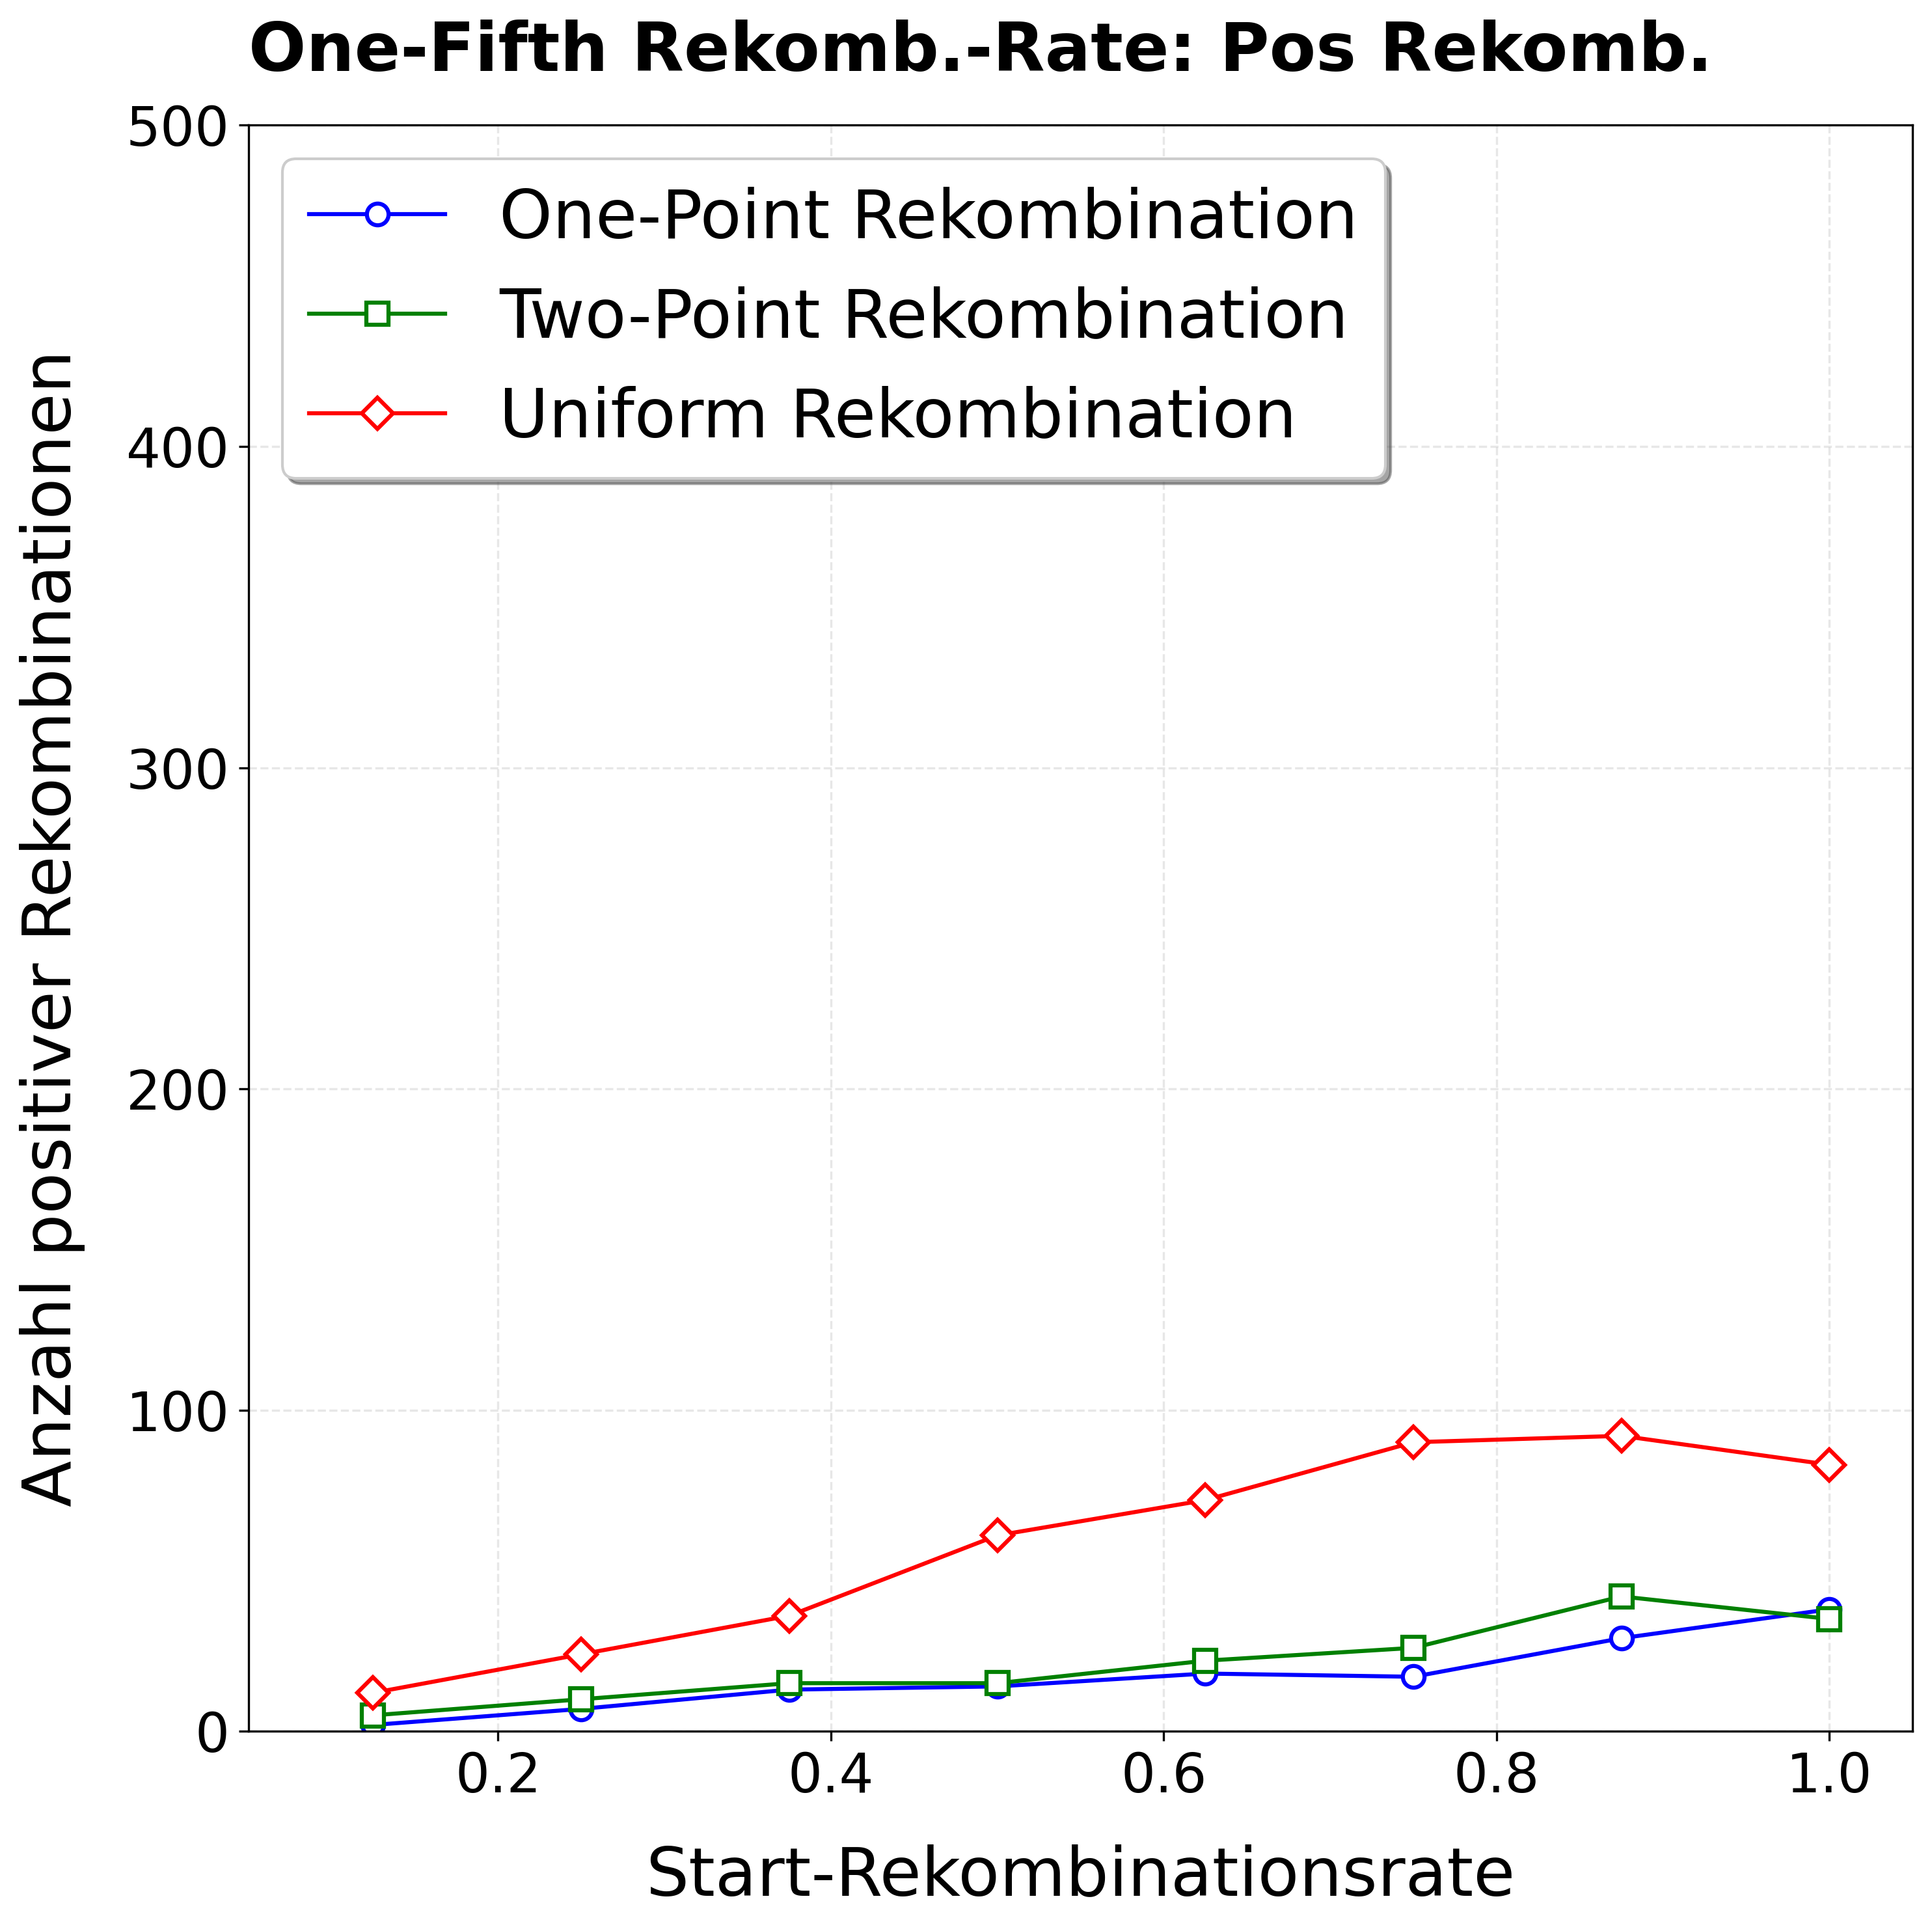
\includegraphics[width=\textwidth]{Bilder/KozaPlotPositiveRekombinationOneFifth.png}
		\caption{One-Fifth Regel}
		\label{fig:kozaPosRekombinationOneFifth}
	\end{subfigure}
	\caption{Koza: Raten-Arten und Anzahl positive Rekombinationen}
	\label{fig:kozaPosRekombination}
\end{figure}

Abbildung \ref{fig:kozaPosRekombination} beschreibt die positiven Rekombinationsraten pro CGP-Konfiguration, aufgeteilt in die verschiedenen Rekombinationsraten-Arten. 
Dabei sind die verschiedenen Rekombinationsarten mit unterschiedlichen Farben dargestellt.
Zu erkennen ist, dass die Uniform Rekombination für jede Rekombinationsraten-Art mehr positive Rekombinationen erzeugt als es die anderen Rekombinationsarten schaffen.
Die Rekombination mit der One-Fifth Regel schneidet in dieser Betrachtung schlechter ab als die konstante und linear fallende Rekombinationsrate.
Zu beachten ist, dass es sich dabei um eine quantitative Bewertung handelt.
Es wird also nicht ersichtlich wie hoch die jeweiligen Trainingserfolge der Rekombinationen ausfallen.
Es macht Sinn dies besonders für SR Benchmarks in weiteren Tests näher zu betrachten, da hier die Fitness einen kontinuierlichen Wert einnimmt und sich die Trainingserfolge stark voneinander unterscheiden können.\\
Für die konstante Rekombinationsrate und diejenige mit der One-Fifth Regel, werden mit höheren Rekombinationsraten auch höhere Chancen gegeben, dass eine Rekombination die Fitness verbessert.
Demnach macht es Sinn, dass für höhere Rekombinationsraten die Anzahl an positiven Rekombinationen steigt, wie es in den Abbildungen \ref{fig:kozaPosRekombinationKonstant} und \ref{fig:kozaPosRekombinationOneFifth} der Fall ist.
Interessant werden demnach diejenigen lokalen Maxima, die bereits entstehen, bevor jeweils die maximale Rekombinationsrate erreicht wurde.
In diesen Punkten könnte die Rekombinationsrate für diese Konfigurationen der Hyperparameter besonders gut ausfallen, da hier prozentual mehr ausgeführte Rekombinationen zu einer Verbesserung der Fitness führen.


\subsection{Rohdatenanalyse: Zusammenfassung}
\label{subsec:rohdatenZusammenfassung}

Zuerst sollen die Ergebnisse der Hyperparameteranalyse von Parity und Keijzer miteinander verglichen werden, um Zusammenhänge zu erschließen und einzelne Beobachtungen validieren zu können.
Die folgenden Abschnitte beziehen sich dabei auf die jeweiligen Spalten der Tabellen \ref{table:parityHPO} und \ref{table:keijzerHPO}.\\
\textbf{Rechenknoten:} Bei Parity kann beobachtet werden, dass die CGP-Konfiguration ohne Rekombination am wenigsten Rechenknoten aufweist. 
Außerdem kann der Trend beobachtet werden, dass komplexere Rekombinationsalgorithmen durchschnittlich weniger Rechenknoten zugeschrieben bekommen als einfachere Algorithmen.
Dabei ist die Streuung um den Mittelwert höher, umso komplexer die Rekombinationsalgorithmen sind.
Dies könnte bedeuten, dass aus einer größeren Rechenknotenanzahl eine kleinere Streuung um diese pro Rekombinationsart folgt.
Im Vergleich dazu ergeben die Ergebnisse von Keijzer ein völlig anderes Bild: gegensätzlich zu Parity hat die CGP-Konfiguration ohne Rekombination die höchste Anzahl an Rechenknoten im Vergleich zu den Mittelwerten über die unterschiedlichen Rekombinationsalgorithmen.
Den bei Parity beobachteten Trend, dass komplexere Rekombinationen eine niedrigere Anzahl an Rechenknoten erfordern könnten, kann bei Keijzer nicht bestätigt werden.
Hier wird für die Uniform-Rekombination die höchste durchschnittliche Anzahl an Rechenknoten erfordert.
Ebenso ergibt sich für Keijzer ein anderes Bild als bei Parity, wenn man die Streuung der Rechenknotenanzahl betrachtet: Die Two-Point Rekombination weist am wenigsten Rechenknoten auf, allerdings auch die geringste Streuung.
Zusammenfassend lässt sich für die Anzahl der Rechenknoten sagen, dass Parity und Keijzer vollkommen unterschiedliche Ergebnisse liefern.
Demnach können keine Aussagen getroffen werden, wie die Anzahl der Rechenknoten mit den unterschiedlichen CGP-Konfigurationen zusammenhängen.
Die Möglichkeit besteht ebenfalls, dass überhaupt kein Zusammenhang zwischen diesen beiden Komponenten besteht.
Durch weitere Tests könnte dies näher betrachtet werden.\\
\textbf{Populationsgröße:} Bei Betrachtung der Populationsgröße kann für Parity zusammengefasst werden, dass die CGP-Konfiguration ohne Rekombination die deutlich kleinste Populationsgröße benötigt hat.
Für Keijzer konnte diese Beobachtung nicht geteilt werden.
Umgekehrt konnte bei Parity nicht bestätigt werden, dass Two-Point und Uniform Rekombination mit linear fallender Rekombinationsrate ohne Offset einen geringeren $\lambda$-Wert aufweisen.
Zusammenfassend lässt sich also auch für die Populationsgröße kein Zusammenhang zu den unterschiedlichen Rekombinationsarten herstellen.\\
\textbf{Rekombinationsraten:} Bei den Ergebnissen der Hyperparameteroptimierung vom Parity-Testszenario werden von konstanten Rekombinationsalgorithmen besonders hohe und besonders niedrige Rekombinationsraten vermieden.
Für die linear fallende Rate und die Rekombinationsrate mit der One-Fifth Regel wird (nahezu) der gesamte Definitionsbereich genutzt.
Wieder im Gegensatz dazu stehen die Ergebnisse des Keijzer-Testszenarios.
Hier werden für nahezu alle CGP-Konfigurationen sehr hohe oder niedrige Werte für die Rekombinationsrate verwendet.
Somit kann durch die Ergebnisse der Hyperparameteranalyse nicht bewertet werden, welche Bereiche der Rekombinationsrate besonders effektiv sind.\\
\textbf{Offset:} Bei Parity wird der geringste Offset bei der Two-Point Rekombination und der höchste Offset bei der Uniform Rekombination verwendet.
Werden bei Keijzer die originalen Ergebnisse verwendet, bei denen ein Offset von 0 zugelassen wird, kann dieses Verhalten ebenfalls beobachtet werden.
Dies könnte bedeuten, dass die Two-Point Rekombination effizienter ist als die Uniform Rekombination, da bei ersterem weniger Rekombinationsschritte ausgesetzt werden.
Die für den Offset neu eingefügten Werte, falls ein Offset gleich 0 bestimmt wird, sind bei Parity ähnlich zum allgemeinen Mittelwert des Offsets.
Ein anderes Verhalten kann für das Keijzer-Testszenario beobachtet werden, bei dem die zweitbesten Parametersätze sehr hohe Offset-Werte verwenden.
Dies ergibt also einen extrem hohen Sprung im Offset zwischen erstbestem und zweitbestem Parametersatz.
Das ist ein Indiz dafür, dass die Güte eines CGPs nicht kausal mit der Höhe des Offsets zusammenhängt.\\
Zu beachten ist, dass die Ergebnisse der Hyperparameteranalyse mit Vorsicht zu begutachten sind.
Um die Ergebnisse und die daraus abgeleiteten Aussagen zu validieren könnte es sinnvoll sein eine umfangreichere Hyperparameteranalyse auszuführen.
Diese sollte mit Hilfe von mehr Rechenkapazität ausgeführt werden, damit mehr Hyperparameter getestet werden können.
Außerdem kann die Anzahl an ausgeführten CGP-Trainings pro Bewertungsschritt in der Hyperparameteranalyse höher gesetzt werden.
Durch diese Schritte könnten sich die Ergebnisse von Parity und Keijzer aneinander angleichen, wodurch bessere Bewertungen stattfinden könnten.
Andernfalls könnte die Aussage gestärkt werden, dass die CGP-Konfigurationen keinen Zusammenhang zur Auswahl einzelner Hyperparameter aufweisen.\\

Folgend sollen die Rohdatenanalysen der vier Testszenarien Parity, Keijzer, Encode und Koza zusammengefasst und miteinander verglichen werden.

Parity:
- Mutation häufiger positiv als Rekombination
- mit Offset keine positive Rekombination + Median Iterationen pos. Rekombinationen
=> Rekombination in frühen Trainingsphasen effizienter
- linear fallende Rekombination bringt hohe Zahlen an pos. Rekombination (wegen hohem Startwert 0,9)
- Konstante Rekombination recht niedrige Werte wegen niedriger Rekombinationsrate 0,3
- One Fifth kaum pos. Rekombinationen 
=> könnte darauf hinweisen, dass One-Fifth keine effiziente Rekombination ergibt
- komplexere Rekombinationsarten machen mehr pos. Rekombinationen
=> kann heißen, dass komplexere Rekombinationen mit höherer Wahrscheinlichkeit Fitness verbessern
=> hohe pos. Rekombinationen können aber auch von hohen Rekombinationsraten aus HPO kommen
- alle Modelle ca. gleich viele Iterationen bis Konvergenz (nicht Clegg am besten wie gedacht) => bedeutet, dass Iterationen bis Konvergenz nicht mit pos. Rekombination zusammenhängt
=> Grund 1: Clegg könnte mehr konvergente Durchläufe haben ohne das man das sehen könnte (ist nicht in Tabelle aufgeführt)
=> Grund 2: negative Mutationen beeinflussen Vorteil aus pos. Rekombinationen
- CGP ohne Rekombination brauchen länger bis Konvergenz (Achtung eingeschränkte Sicht, weil nur die konvergenten Iterationen einbezogen werden und nicht wie viele CGP konvergieren)
=> kann trotzdem darauf hinweisen, dass es sich lohnen kann Rekombination auszuführen
=> Bayes und Graphen müssen mehr Infos bringen
- 7 aus 9 Offsets aktiviert, obwohl diese Rekombination blockieren -> wieso?
=> HPO hätte evtl mehr Parametersätze testen sollen
=> Offset im Zusammenhang mit negativen Mutationen -> negative Mutationen machen nicht nur pos. Rekombinationen kaputt, sondern verhindern auch lernen mit Mutation (also ist am Ende "keine Rekombination", weil dann wenigsten Mutation klappt)
- Uniform hat viel Offset und auch viel neg. Mutation (+ Offset bei Uniform war nie gleich 0 in HPO)




TODO: Argumentation bezüglich Offset von Encode doch in praktischen Teil packen
TODO: Argumentation; dass Offset nicht so viel bringt (damit Kapitel \glqq praktischer Teil\grqq\space darauf verweisen kann)\\
- HPO: mehrere Durchläufe wählen garkeinen Offset\\
- restliche Tests vergleichen zwischen mit Offset und ohne\\
- Rohdatenanalyse: Rekombinationserfolge; wenn kein Offset da ist


TODO: Wieso wurde Offset überhaupt in HPO Ergebnissen (7 aus 9) verwendet?

TODO: Encode und Koza Ergebnisse mit Vorsicht betrachten: Hier wurden für "keine Rekombination" eine HPO ausgeführt und für Rest nicht





\section{Ergebnisse Bayes'sche Analyse}
\label{sec:ergebnisseBayes}

\subsection{Bayes'sche Analyse: Parity}
\label{subsec:bayesParity}

\begin{table}[H]
	\centering
	\begin{tabular}{c | c | c | c}
		\textbf{CPG-Konfiguration} & \textbf{HPDI (Iter.)} & \textbf{MW} & \textbf{PL-Platz}\\
		\hline
		Parity keine Rekombination & (237,958; 541,181) & 357,440 & 0,034518\\
		\hline
		Parity One-Point Konstant kein Offset & (72,803; 131,161) & 98,059 & 0,072723\\
		\hline
		Parity One-Point Konstant mit Offset & (117,5867; 241,124) & 168,301 & 0,059872\\
		\hline
		Parity One-Point Clegg kein Offset & (111,330; 204,672) & 151,207 & 0,058134\\
		\hline
		Parity One-Point Clegg mit Offset & (136,755; 318,250) & 208,318 & 0,064637\\
		\hline
		Parity One-Point One-Fifth kein Offset & (305,150; 879,234) & 516,320 & 0,041265\\
		\hline
		Parity One-Point One-Fifth mit Offset & (90,584; 192,603) & 132,238 & 0,072643\\
		\hline
		Parity Two-Point Konstant kein Offset & (161,166; 366,726) & 243,306 & 0,056980\\
		\hline
		Parity Two-Point Konstant mit Offset & (185,680; 398,045) & 271,755 & 0,043839\\
		\hline
		Parity Two-Point Clegg kein Offset & (143,411; 320,218) & 214,015 & 0,055768\\
		\hline
		Parity Two-Point Clegg mit Offset & (279,211; 671,061) & 429,804 & 0,041189\\
		\hline
		Parity Two-Point One-Fifth kein Offset & (165,870; 369,988) & 247,230 & 0,051913\\
		\hline
		Parity Two-Point One-Fifth mit Offset & (187,841; 467,866) & 294,748 & 0,049240\\
		\hline
		Parity Uniform Konstant kein Offset & (182,312; 414,373) & 275,283 & 0,043305\\
		\hline
		Parity Uniform Konstant mit Offset & (158,116; 357,830) & 238,048 & 0,060934\\
		\hline
		Parity Uniform Clegg kein Offset & (120,352; 267,732) & 179,796 & 0,063633\\
		\hline
		Parity Uniform Clegg mit Offset & (147,184; 317,828) & 215,359 & 0,051520\\
		\hline
		Parity Uniform One-Fifth kein Offset & (233,817; 551,718) & 356,681 & 0,040460\\
		\hline
		Parity Uniform One-Fifth mit Offset & (211,377; 519,471) & 329,524 & 0,037426\\
	\end{tabular}
	\label{table:parityBayesian}
	\caption{Parity: Bayes'sche Analyse}
\end{table}

\subsection{Bayes'sche Analyse: Keijzer}
\label{subsec:bayesKeijzer}

\begin{table}[H]
	\centering
	\begin{tabular}{c | c | c | c}
		\textbf{CGP-Konfiguration} & \textbf{HPDI (Iter.)} & \textbf{MW} & \textbf{PL-Platz}\\
		\hline
		Keijzer keine Rekombination & (5446,690; 16772,637) & 9551,657 & 0,046669\\
		\hline
		Keijzer One-Point Konstant kein Offset & (3155,154; 8685,286) & 5214,911 & 0,056954\\
		\hline
		Keijzer One-Point Konstant mit Offset & (5791,946; 19545,587) & 10837,605 & 0,047578\\
		\hline
		Keijzer One-Point Clegg kein Offset & (4055,470; 14388,586) & 7754,999 & 0,053452\\
		\hline
		Keijzer One-Point Clegg mit Offset & (5182,282; 17954,643) & 9757,394 & 0,046700\\
		\hline
		Keijzer One-Point One-Fifth kein Offset & (3746,883; 10479,686) & 6233,279 & 0,050072\\
		\hline
		Keijzer One-Point One-Fifth mit Offset & (4972,228; 16087,780) & 9402,618 & 0,057995\\
		\hline
		Keijzer Two-Point Konstant kein Offset & (4207,924; 13285,672) & 7464,243 & 0,061749\\
		\hline
		Keijzer Two-Point Konstant mit Offset & (3544,144; 10355,412) & 6056,680 & 0,064480\\
		\hline
		Keijzer Two-Point Clegg kein Offset & (5468,641; 17877,607) & 10017,892 & 0,033887\\
		\hline
		Keijzer Two-Point Clegg mit Offset & (4105,772; 13578,136) & 7663,952 & 0,055730\\
		\hline
		Keijzer Two-Point One-Fifth kein Offset & (4408,582; 12408,349) & 7381,426 & 0,053392\\
		\hline
		Keijzer Two-Point One-Fifth mit Offset & (6970,619; 22911,685) & 13432,511 & 0,052018\\
		\hline
		Keijzer Uniform Konstant kein Offset & (8010,603; 23268,991) & 14688,052 & 0,049104\\
		\hline
		Keijzer Uniform Konstant mit Offset & (3406,437; 10751,973) & 6052,727 & 0,069820\\
		\hline
		Keijzer Uniform Clegg kein Offset & (3856,791; 10850,478) & 6440,975 & 0,060934\\
		\hline
		Keijzer Uniform Clegg mit Offset & (6067,492; 20498,984) & 11238,547 & 0,043535\\
		\hline
		Keijzer Uniform One-Fifth kein Offset & (3511,828; 12119,350) & 6587,897 & 0,070569\\
		\hline
		Keijzer Uniform One-Fifth mit Offset & (4025,084; 11844,356) & 6893,370 & 0,025362\\
	\end{tabular}
	\label{table:keijzerBayesian}
	\caption{Keijzer: Bayes'sche Analyse}
\end{table}

\subsection{Bayes'sche Analyse: Encode}
\label{subsec:bayesEncode}

\begin{table}[H]
	\centering
	\begin{tabular}{c | c | c | c}
		\textbf{CGP-Konfiguration} & \textbf{HPDI (Fitn.)} & \textbf{MW} & \textbf{PL-Platz}\\
		\hline
		Encode keine Rekombination & (0,02727; 0,06853) & 0,04351 & 0,040300\\
		\hline
		Encode One-Point Konstant: 0,125 & (0,02416; 0,06463) & 0,03969 & 0,039235\\
		\hline
		Encode One-Point Konstant: 0,25 & (0,02342; 0,06255) & 0,03837 & 0,044399\\
		\hline
		Encode One-Point Konstant: 0,375 & (0,02216; 0,05684) & 0,036 & 0,052266\\
		\hline
		Encode One-Point Konstant: 0,5 & (0,02581; 0,06657) & 0,04185 & 0,041112\\
		\hline
		Encode One-Point Konstant: 0,625 & (0,02703; 0,06417) & 0,04188 & 0,039622\\
		\hline
		Encode One-Point Konstant: 0,75 & (0,02484; 0,05755) & 0,03791 & 0,047276\\
		\hline
		Encode One-Point Konstant: 0,875 & (0,02311; 0,06519) & 0,03911 & 0,042973\\
		\hline
		Encode One-Point Konstant: 1,0 & (0,02634; 0,06865) & 0,04257 & 0,040402\\
		\hline
		Encode One-Point Clegg: 0,0005 & (0,01874; 0,05612) & 0,03254 & 0,058275\\
		\hline
		Encode One-Point Clegg: 0,0015 & (0,03085; 0,07312) & 0,04756 & 0,033251\\
		\hline
		Encode One-Point Clegg: 0,0025 & (0,03174; 0,07112) & 0,04783 & 0,036894\\
		\hline
		Encode One-Point Clegg: 0,0035 & (0,0259; 0,05957) & 0,03961 & 0,043415\\
		\hline
		Encode One-Point Clegg: 0,0045 & (0,02262; 0,05981) & 0,03682 & 0,047645\\
		\hline
		Encode One-Point Clegg: 0,0055 & (0,02478; 0,06459) & 0,04044 & 0,044801\\
		\hline
		Encode One-Point One-Fifth: 0,125 & (0,02234; 0,06005) & 0,03702 & 0,048045\\
		\hline
		Encode One-Point One-Fifth: 0,25 & (0,02132; 0,06241) & 0,0368 & 0,053389\\
		\hline
		Encode One-Point One-Fifth: 0,375 & (0,02423; 0,05867) & 0,03784 & 0,049249\\
		\hline
		Encode One-Point One-Fifth: 0,5 & (0,01903; 0,05371) & 0,03227 & 0,060271\\
		\hline
		Encode One-Point One-Fifth: 0,625 & (0,02184; 0,0643) & 0,03777 & 0,045892\\
		\hline
		Encode One-Point One-Fifth: 0,75 & (0,02746; 0,06625) & 0,04286 & 0,041786\\
		\hline
		Encode One-Point One-Fifth: 0,875 & (0,02436; 0,05364) & 0,03622 & 0,049501\\
	\end{tabular}
	\label{table:encodeOnePointBayesian}
	\caption{Encode One-Point Rekombination: Bayes'sche Analyse}
\end{table}

\begin{table}[H]
	\centering
	\begin{tabular}{c | c | c | c}
		\textbf{CGP-Konfiguration} & \textbf{HPDI (Fitn.)} & \textbf{MW} & \textbf{PL-Platz}\\
		\hline
		Encode keine Rekombination & (0,02727; 0,06853) & 0,04351 & 0,064969\\
		\hline
		Encode Two-Point Konstant: 0,125 & (0,04657; 0,08164) & 0,06176 & 0,036705\\
		\hline
		Encode Two-Point Konstant: 0,25 & (0,0417; 0,08229) & 0,05853 & 0,038448\\
		\hline
		Encode Two-Point Konstant: 0,375 & (0,03172; 0,07007) & 0,04742 & 0,056475\\
		\hline
		Encode Two-Point Konstant: 0,5 & (0,04318; 0,08532) & 0,06094 & 0,037807\\
		\hline
		Encode Two-Point Konstant: 0,625 & (0,03854; 0,07511) & 0,05397 & 0,047998\\
		\hline
		Encode Two-Point Konstant: 0,75 & (0,05211; 0,08389) & 0,06618 & 0,035496\\
		\hline
		Encode Two-Point Konstant: 0,875 & (0,03614; 0,08027) & 0,05438 & 0,045400\\
		\hline
		Encode Two-Point Konstant: 1,0 & (0,03386; 0,07925) & 0,052 & 0,047936\\
		\hline
		Encode Two-Point Clegg: 0,0005 & (0,03588; 0,07852) & 0,05322 & 0,046264\\
		\hline
		Encode Two-Point Clegg: 0,0015 & (0,0457; 0,08078) & 0,06077 & 0,036224\\
		\hline
		Encode Two-Point Clegg: 0,0025 & (0,03801; 0,07255) & 0,05258 & 0,050576\\
		\hline
		Encode Two-Point Clegg: 0,0035 & (0,04651; 0,09123) & 0,06523 & 0,034689\\
		\hline
		Encode Two-Point Clegg: 0,0045 & (0,0321; 0,07079) & 0,04795 & 0,054090\\
		\hline
		Encode Two-Point Clegg: 0,0055 & (0,03634; 0,08965) & 0,0573 & 0,039299\\
		\hline
		Encode Two-Point One-Fifth: 0,125 & (0,04561; 0,08148) & 0,06082 & 0,042431\\
		\hline
		Encode Two-Point One-Fifth: 0,25 & (0,04353; 0,0687) & 0,05485 & 0,047932\\
		\hline
		Encode Two-Point One-Fifth: 0,375 & (0,04642; 0,07558) & 0,05903 & 0,041419\\
		\hline
		Encode Two-Point One-Fifth: 0,5 & (0,03834; 0,07567) & 0,0539 & 0,045002\\
		\hline
		Encode Two-Point One-Fifth: 0,625 & (0,036; 0,07918) & 0,0536 & 0,047777\\
		\hline
		Encode Two-Point One-Fifth: 0,75 & (0,03114; 0,07277) & 0,04805 & 0,053331\\
		\hline
		Encode Two-Point One-Fifth: 0,875 & (0,03244; 0,07634) & 0,05012 & 0,049732\\
	\end{tabular}
	\label{table:encodeTwoPointBayesian}
	\caption{Encode Two-Point Rekombination: Bayes'sche Analyse}
\end{table}

\begin{table}[H]
	\centering
	\begin{tabular}{c | c | c | c}
		\textbf{CGP-Konfiguration} & \textbf{HPDI (Fitn.)} & \textbf{MW} & \textbf{PL-Platz}\\
		\hline
		Encode keine Rekombination & (0,02727; 0,06853) & 0,04351 & 0,037060\\
		\hline
		Encode Uniform Konstant: 0,125 & (0,02473; 0,06504) & 0,04031 & 0,038501\\
		\hline
		Encode Uniform Konstant: 0,25 & (0,02356; 0,06581) & 0,03963 & 0,040006\\
		\hline
		Encode Uniform Konstant: 0,375 & (0,03039; 0,07186) & 0,047 & 0,034479\\
		\hline
		Encode Uniform Konstant: 0,5 & (0,02241; 0,05759) & 0,03583 & 0,050278\\
		\hline
		Encode Uniform Konstant: 0,625 & (0,02416; 0,05673) & 0,03719 & 0,046887\\
		\hline
		Encode Uniform Konstant: 0,75 & (0,02399; 0,06258) & 0,03882 & 0,050394\\
		\hline
		Encode Uniform Konstant: 0,875 & (0,02203; 0,05148) & 0,03393 & 0,052041\\
		\hline
		Encode Uniform Konstant: 1,0 & (0,022; 0,05696) & 0,03592 & 0,048403\\
		\hline
		Encode Uniform Clegg: 0,0005 & (0,01801; 0,0552) & 0,03171 & 0,053799\\
		\hline
		Encode Uniform Clegg: 0,0015 & (0,02101; 0,06014) & 0,03576 & 0,052238\\
		\hline
		Encode Uniform Clegg: 0,0025 & (0,01737; 0,04703) & 0,02884 & 0,057695\\
		\hline
		Encode Uniform Clegg: 0,0035 & (0,02831; 0,05921) & 0,04102 & 0,041420\\
		\hline
		Encode Uniform Clegg: 0,0045 & (0,0247; 0,06962) & 0,04197 & 0,037226\\
		\hline
		Encode Uniform Clegg: 0,0055 & (0,02211; 0,05691) & 0,03563 & 0,044593\\
		\hline
		Encode Uniform One-Fifth: 0,125 & (0,02138; 0,05172) & 0,03338 & 0,046835\\
		\hline
		Encode Uniform One-Fifth: 0,25 & (0,02075; 0,06059) & 0,03566 & 0,046254\\
		\hline
		Encode Uniform One-Fifth: 0,375 & (0,02667; 0,06216) & 0,04111 & 0,039581\\
		\hline
		Encode Uniform One-Fifth: 0,5 & (0,01608; 0,04588) & 0,02738 & 0,063355\\
		\hline
		Encode Uniform One-Fifth: 0,625 & (0,02459; 0,06074) & 0,03881 & 0,048598\\
		\hline
		Encode Uniform One-Fifth: 0,75 & (0,02107; 0,06167) & 0,03642 & 0,042721\\
		\hline
		Encode Uniform One-Fifth: 0,875 & (0,03182; 0,07718) & 0,04969 & 0,027637\\
	\end{tabular}
	\label{table:encodeUniformBayesian}
	\caption{Encode Uniform Rekombination: Bayes'sche Analyse}
\end{table}

\subsection{Bayes'sche Analyse: Koza}
\label{subsec:bayesKoza}

\begin{table}[H]
	\centering
	\begin{tabular}{c | c | c | c}
		\textbf{CPG-Konfiguration} & \textbf{HPDI (Iter.)} & \textbf{MW} & \textbf{PL-Platz}\\
		\hline
		Koza keine Rekombination & (3306,396; 9338,152) & 5573,228 & 0,066044\\
		\hline
		Koza One-Point Konstant: 0,125 & (11989,955; 39904,351) & 22076,286 & 0,039745\\
		\hline
		Koza One-Point Konstant: 0,25 & (5686,475; 17041,592) & 9857,749 & 0,053368\\
		\hline
		Koza One-Point Konstant: 0,375 & (7670,190; 19745,987) & 12308,128 & 0,041433\\
		\hline
		Koza One-Point Konstant: 0,5 & (21220,641; 77451,788) & 41120,883 & 0,030037\\
		\hline
		Koza One-Point Konstant: 0,625 & (8850,276; 22781,194) & 14213,974 & 0,042111\\
		\hline
		Koza One-Point Konstant: 0,75 & (6558,793; 17538,734) & 10732,756 & 0,050455\\
		\hline
		Koza One-Point Konstant: 0,875 & (22884,073; 83707,754) & 44778,187 & 0,034913\\
		\hline
		Koza One-Point Konstant: 1,0 & (11999,809; 40932,104) & 22223,655 & 0,045110\\
		\hline
		Koza One-Point Clegg: 0,0005 & (8804,961; 28842,331) & 16070,796 & 0,046374\\
		\hline
		Koza One-Point Clegg: 0,0015 & (12897,221; 44229,228) & 24132,461 & 0,034105\\
		\hline
		Koza One-Point Clegg: 0,0025 & (12097,518; 42109,886) & 22745,754 & 0,042530\\
		\hline
		Koza One-Point Clegg: 0,0035 & (10713,692; 36149,781) & 19751,179 & 0,041706\\
		\hline
		Koza One-Point Clegg: 0,0045 & (8152,673; 25944,800) & 14620,549 & 0,050148\\
		\hline
		Koza One-Point Clegg: 0,0055 & (10396,968; 32228,793) & 18312,576 & 0,045403\\
		\hline
		Koza One-Point One-Fifth: 0,125 & (7042,406; 22949,117) & 12782,824 & 0,055561\\
		\hline
		Koza One-Point One-Fifth: 0,25 & (8698,915; 24772,687) & 14733,520 & 0,046146\\
		\hline
		Koza One-Point One-Fifth: 0,375 & (5766,106; 16551,173) & 9801,340 & 0,052473\\
		\hline
		Koza One-Point One-Fifth: 0,5 & (10523,665; 39039,177) & 20390,489 & 0,048112\\
		\hline
		Koza One-Point One-Fifth: 0,625 & (7477,611; 22329,849) & 13015,454 & 0,043730\\
		\hline
		Koza One-Point One-Fifth: 0,75 & (9605,964; 28910,079) & 16579,745 & 0,046481\\
		\hline
		Koza One-Point One-Fifth: 0,875 & (7844,463; 27078,528) & 14728,439 & 0,044015\\
	\end{tabular}
	\label{table:kozaOnePointBayesian}
	\caption{Koza One-Point Rekombination: Bayes'sche Analyse}
\end{table}

\begin{table}[H]
	\centering
	\begin{tabular}{c | c | c | c}
		\textbf{CPG-Konfiguration} & \textbf{HPDI (Iter.)} & \textbf{MW} & \textbf{PL-Platz}\\
		\hline
		Koza keine Rekombination & (3306,396; 9338,152) & 5573,228 & 0,044276\\
		\hline
		Koza Two-Point Konstant: 0,125 & (5778,032; 20659,534) & 11104,449 & 0,050079\\
		\hline
		Koza Two-Point Konstant: 0,25 & (4377,352; 12699,617) & 7467,417 & 0,043383\\
		\hline
		Koza Two-Point Konstant: 0,375 & (7682,846; 29668,729) & 15237,451 & 0,042903\\
		\hline
		Koza Two-Point Konstant: 0,5 & (4545,700; 15211,867) & 8448,030 & 0,047157\\
		\hline
		Koza Two-Point Konstant: 0,625 & (2506,268; 7690,605) & 4414,865 & 0,052680\\
		\hline
		Koza Two-Point Konstant: 0,75 & (8106,535; 30489,526) & 15831,484 & 0,036253\\
		\hline
		Koza Two-Point Konstant: 0,875 & (5275,995; 16141,930) & 9274,253 & 0,039958\\
		\hline
		Koza Two-Point Konstant: 1,0 & (2467,382; 7467,193) & 4300,790 & 0,058410\\
		\hline
		Koza Two-Point Clegg: 0,0005 & (3539,092; 10910,749) & 6214,133 & 0,046851\\
		\hline
		Koza Two-Point Clegg: 0,0015 & (5136,595; 18389,726) & 9803,362 & 0,040274\\
		\hline
		Koza Two-Point Clegg: 0,0025 & (7068,983; 23388,559) & 12866,463 & 0,039712\\
		\hline
		Koza Two-Point Clegg: 0,0035 & (4920,069; 17123,138) & 9196,381 & 0,052770\\
		\hline
		Koza Two-Point Clegg: 0,0045 & (5065,402; 17637,588) & 9552,405 & 0,049098\\
		\hline
		Koza Two-Point Clegg: 0,0055 & (2005,714; 5792,200) & 3420,063 & 0,059170\\
		\hline
		Koza Two-Point One-Fifth: 0,125 & (5549,634; 19765,485) & 10495,382 & 0,042831\\
		\hline
		Koza Two-Point One-Fifth: 0,25 & (8535,956; 28712,980) & 15794,048 & 0,033087\\
		\hline
		Koza Two-Point One-Fifth: 0,375 & (6383,072; 19877,145) & 11333,015 & 0,033814\\
		\hline
		Koza Two-Point One-Fifth: 0,5 & (4715,287; 13037,660) & 7854,211 & 0,034314\\
		\hline
		Koza Two-Point One-Fifth: 0,625 & (3209,936; 9921,136) & 5663,114 & 0,051706\\
		\hline
		Koza Two-Point One-Fifth: 0,75 & (4615,524; 15765,276) & 8647,855 & 0,047033\\
		\hline
		Koza Two-Point One-Fifth: 0,875 & (2480,371; 7460,089) & 4313,097 & 0,054242\\
	\end{tabular}
	\label{table:kozaTwoPointBayesian}
	\caption{Koza Two-Point Rekombination: Bayes'sche Analyse}
\end{table}


\begin{table}[H]
	\centering
	\begin{tabular}{c | c | c | c}
		\textbf{CPG-Konfiguration} & \textbf{HPDI (Iter.)} & \textbf{MW} & \textbf{PL-Platz}\\
		\hline
		Koza keine Rekombination & (3306,396; 9338,152) & 5573,228 & 0,046653\\
		\hline
		Koza Uniform Konstant: 0,125 & (7116,082; 25435,336) & 13593,719 & 0,038759\\
		\hline
		Koza Uniform Konstant: 0,25 & (9984,851; 33237,558) & 18247,622 & 0,032483\\
		\hline
		Koza Uniform Konstant: 0,375 & (3172,788; 9799,001) & 5586,763 & 0,054234\\
		\hline
		Koza Uniform Konstant: 0,5 & (5845,776; 21080,773) & 11192,410 & 0,048150\\
		\hline
		Koza Uniform Konstant: 0,625 & (5056,513; 15161,941) & 8855,128 & 0,044384\\
		\hline
		Koza Uniform Konstant: 0,75 & (7678,984; 28599,746) & 14989,121 & 0,042284\\
		\hline
		Koza Uniform Konstant: 0,875 & (8075,534; 25962,001) & 14529,689 & 0,037376\\
		\hline
		Koza Uniform Konstant: 1,0 & (6997,916; 26553,700) & 13799,512 & 0,050811\\
		\hline
		Koza Uniform Clegg: 0,0005 & (5887,321; 17725,061) & 10263,6346 & 0,039935\\
		\hline
		Koza Uniform Clegg: 0,0015 & (1820,854; 5880,233) & 3284,824 & 0,070103\\
		\hline
		Koza Uniform Clegg: 0,0025 & (2105,563; 6348,965) & 3669,648 & 0,062192\\
		\hline
		Koza Uniform Clegg: 0,0035 & (6267,561; 20173,041) & 11336,109 & 0,042816\\
		\hline
		Koza Uniform Clegg: 0,0045 & (3259,699; 8595,464) & 5275,119 & 0,045873\\
		\hline
		Koza Uniform Clegg: 0,0055 & (4447,802; 15210,844) & 8263,146 & 0,047253\\
		\hline
		Koza Uniform One-Fifth: 0,125 & (9555,821; 36197,611) & 18956,129 & 0,041516\\
		\hline
		Koza Uniform One-Fifth: 0,25 & (6369,195; 24041,614) & 12519,802 & 0,045399\\
		\hline
		Koza Uniform One-Fifth: 0,375 & (4284,718; 13099,952) & 7548,330 & 0,045936\\
		\hline
		Koza Uniform One-Fifth: 0,5 & (6205,669; 18180,546) & 10642,776 & 0,039174\\
		\hline
		Koza Uniform One-Fifth: 0,625 & (5184,311; 15589,695) & 9047,982 & 0,039264\\
		\hline
		Koza Uniform One-Fifth: 0,75 & (7626,548; 26532,940) & 14283,760 & 0,040292\\
		\hline
		Koza Uniform One-Fifth: 0,875 & (4522,053; 14978,774) & 8243,582 & 0,045112\\
	\end{tabular}
	\label{table:kozaUniformBayesian}
	\caption{Koza Uniform Rekombination: Bayes'sche Analyse}
\end{table}

\subsection{Bayes'sche Analyse: Zusammenfassung}
\label{subsec:bayesZusammenfassung}

\section{Ergebnisse Graphische Evaluation}
\label{sec:ergebnissePlots}

\subsection{Graphische Evaluation: Parity}
\label{subsec:plotsParity}

\subsection{Graphische Evaluation: Keijzer}
\label{subsec:plotsKeijzer}

\subsection{Graphische Evaluation: Encode}
\label{subsec:plotsEncode}

\subsection{Graphische Evaluation: Koza}
\label{subsec:plotsKoza}

\subsection{Graphische Evaluation: Zusammenfassung}
\label{subsec:plotsZusammenfassung}
